\documentclass[11pt,a4paper]{article}
\newcommand{\simname}{Piezopeening Coverage Simulator}
\usepackage[utf8]{inputenc}
\usepackage[T1]{fontenc}
\usepackage[sc]{mathpazo}
\linespread{1.05}
\usepackage[english]{babel}
\usepackage[margin=2.2cm]{geometry}
\usepackage{amsmath,amssymb}
\usepackage[locale=UK,per-mode=symbol]{siunitx}
\usepackage{booktabs,array,tabularx,longtable}
\usepackage{graphicx}
\usepackage{tikz}
\usetikzlibrary{arrows.meta,decorations.pathreplacing,calc}
\usepackage{xcolor}
\usepackage[hidelinks]{hyperref}
\usepackage{enumitem}
\usepackage{tcolorbox}
\usepackage{float}
\usepackage[font=small,labelfont=bf]{caption}
\usepackage{subcaption}
\usepackage{fancyhdr}
\usepackage{multicol}

\definecolor{bleu}{HTML}{1F5A96}
\definecolor{orange}{HTML}{D4621C}
\definecolor{vert}{HTML}{2E8B57}
\definecolor{rouge}{HTML}{E5484D}
\newtcolorbox{keybox}[1][]{colback=bleu!5,colframe=bleu,boxrule=0.6pt,arc=2pt,left=6pt,right=6pt,top=4pt,bottom=4pt,#1}
\newtcolorbox{trybox}[1][]{colback=orange!6,colframe=orange,boxrule=0.6pt,arc=2pt,left=6pt,right=6pt,top=4pt,bottom=4pt,#1}
\newcommand{\E}{\mathbb{E}}
\newcommand{\dX}{\Delta X}
\newcommand{\ui}[1]{\textsf{#1}}   % name of a control or a readout on the page
\setlength{\tabcolsep}{5pt}
\renewcommand{\arraystretch}{1.15}

\pagestyle{fancy}
\fancyhf{}
\fancyhead[L]{\small Dr Régis Kubler, Arts et Métiers Institute of Technology}
\fancyhead[R]{\small\simname}
\fancyfoot[C]{\small\thepage}
\renewcommand{\headrulewidth}{0.4pt}
\setlength{\headheight}{14pt}
\setlength{\parskip}{3pt}
\usepackage{newunicodechar}
\newunicodechar{λ}{\ensuremath{\lambda}}
\newunicodechar{Σ}{\ensuremath{\Sigma}}
\newunicodechar{Δ}{\ensuremath{\Delta}}
\newunicodechar{δ}{\ensuremath{\delta}}
\newunicodechar{τ}{\ensuremath{\tau}}
\newunicodechar{σ}{\ensuremath{\sigma}}
\newunicodechar{η}{\ensuremath{\eta}}
\newunicodechar{α}{\ensuremath{\alpha}}
\newunicodechar{φ}{\ensuremath{\varphi}}
\newunicodechar{ζ}{\ensuremath{\zeta}}
\newunicodechar{²}{\ensuremath{^2}}
\newunicodechar{³}{\ensuremath{^3}}
\newunicodechar{−}{\ensuremath{-}}
\newunicodechar{·}{\ensuremath{\cdot}}
\newunicodechar{×}{\ensuremath{\times}}
\newunicodechar{≈}{\ensuremath{\approx}}
\newunicodechar{≥}{\ensuremath{\geq}}
\newunicodechar{≤}{\ensuremath{\leq}}
\newunicodechar{→}{\ensuremath{\rightarrow}}
\newunicodechar{°}{\ensuremath{^\circ}}
\newunicodechar{µ}{\ensuremath{\mu}}
\newunicodechar{…}{\ldots}
\newunicodechar{ṁ}{\ensuremath{\dot m}}
\newunicodechar{Ṅ}{\ensuremath{\dot N}}
\newunicodechar{₀}{\ensuremath{_0}}
\newunicodechar{₉}{\ensuremath{_9}}
\newunicodechar{₈}{\ensuremath{_8}}
\newunicodechar{₅}{\ensuremath{_5}}

\newunicodechar{₁}{\ensuremath{_1}}

\title{\textbf{Piezopeening Coverage Simulator}\\[3pt]
\large User and theory guide: dents made by a vibrating spherical tool moved along CNC lines}
\author{Dr Régis Kubler\\ Arts et Métiers Institute of Technology\\[4pt]
\small Developed with the assistance of Claude Opus 5.5 (Anthropic), November 2026}
\date{Guide for simulator version 2.0 (18 November 2026)\\ \url{https://rkubler.github.io/piezopeening-coverage/}}

\begin{document}
\maketitle
\thispagestyle{fancy}

\begin{abstract}
\noindent This guide explains the Piezopeening Coverage Simulator. It starts with the basic idea and a first experiment, then explains the motion of the tool, the shape of one dent, the regular lattice of impacts, the number of hits per point, the depth of the dents and the waviness of the surface, and the comparison with random (shot peening) impacts, the 2D and 3D roughness of the treated surface, and the coverage above 100\,\% of NF~L~06-832. Every parameter, every result and every chart displayed on the page is listed with its formula and its default value.
\end{abstract}

\tableofcontents

\section{The idea in one page}

\paragraph{Piezopeening.} A piezoelectric actuator drives a hard spherical tool up and down at a frequency $f$ (typically 100 Hz to a few kHz), while a CNC machine moves it along straight lines at the feed velocity $V$. Each time the tool goes below the initial surface it indents it. Instead of millions of shots landing at random, as in shot peening, the dents are placed on a \emph{regular lattice}: a spacing $s=V/f$ along each line, and a step-over $p$ between lines.

\paragraph{What the page computes.} The page follows the tool, stamps every dent on a fine grid of the treated zone, and counts how many times each point is hit. From these counts it gives the measured coverage (share of the zone with at least one dent), the distribution of hits, the depth map of the surface and its waviness, and it compares the result with a random process that has the same number of dents per mm², as shot peening would.

\begin{trybox}
\textbf{First experiment.} The page opens with a tool of diameter \SI{3}{mm}, $f=\SI{100}{Hz}$, amplitude $a=\SI{40}{\micro m}$, median line $U_\mathrm{off}=\SI{20}{\micro m}$ inside the material, $V=\SI{16.7}{mm/s}$ and a step-over $p=\SI{0.8}{mm}$. Press \ui{Play}: the tool hits the surface every \SI{167}{\micro m}; seven lines later (\ui{Run all}):
\begin{itemize}[nosep]
\item each dent has a radius of \SI{420}{\micro m} and is round ($L/W=1.01$);
\item the measured zone is \SI{100}{\percent} covered with 238 impacts; every point is hit between 2 and 6 times, 4.17 on average;
\item 98\,\% of the zone is dented after 0.96 pass (the base time), so the coverage according to NF~L~06-832 is \SI{98.3}{\percent} after one pass and 249\,\% after three passes (Section~\ref{sec:nf});
\item a random process with the same mean would leave \SI{1.5}{\percent} of the surface untouched and spread the hits from 0 to 14;
\end{itemize}
Then set $p=\SI{1.2}{mm}$: strips between the lines stay untouched and the coverage drops to \SI{71}{\percent}.
\end{trybox}

\section{The screen}

\begin{figure}[H]
\centering
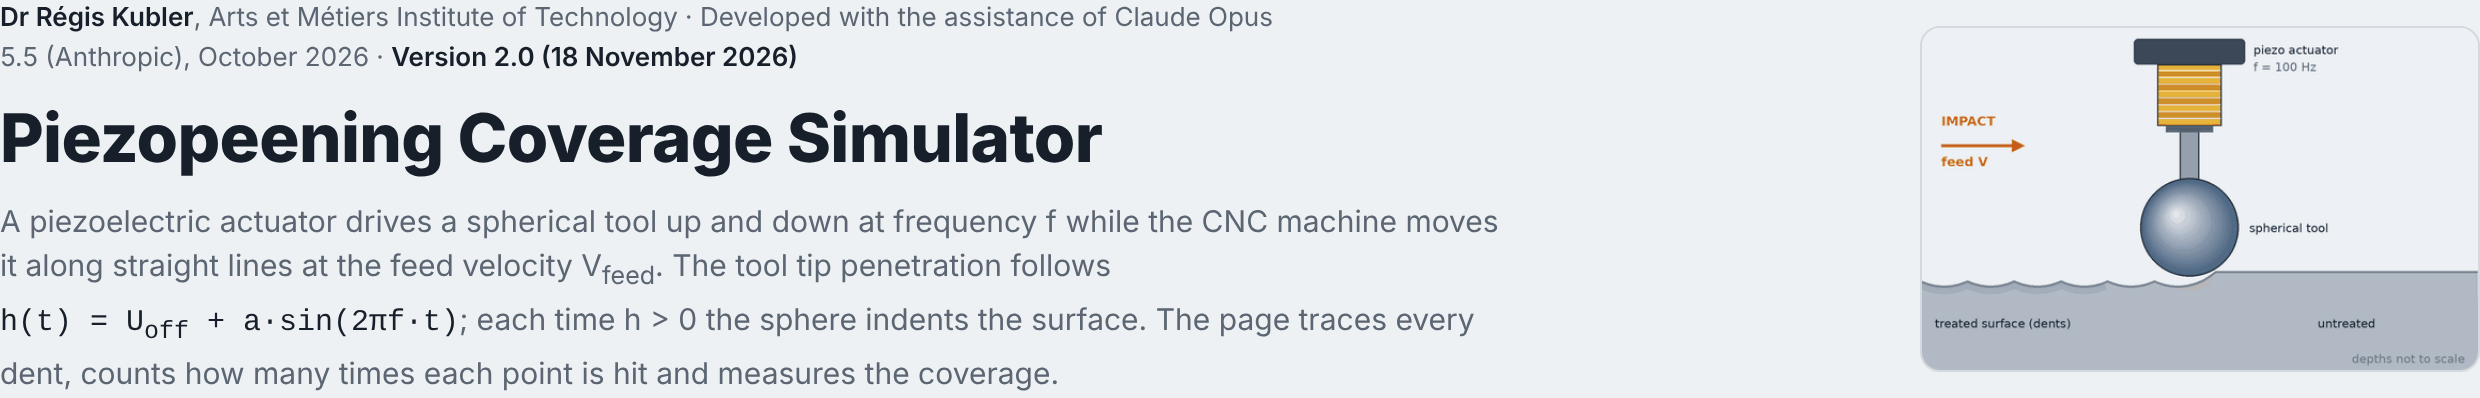
\includegraphics[width=\linewidth]{img/header.png}\\[2pt]

\includegraphics[width=\linewidth]{img/toolbar.png}
\caption{Header (with the kinematic law) and toolbar.}
\end{figure}

\paragraph{Toolbar.}
\begin{description}[leftmargin=2.6cm,style=nextline,itemsep=2pt]
\item[\ui{Play / Pause}] moves the tool along the lines (\ui{Replay} at the end).
\item[\ui{+1 line}] travels exactly one more line and stops.
\item[\ui{Run all}] makes all the lines of all the passes at once.
\item[\ui{Restart}] clears the zone.
\item[\ui{Animation speed}] $\times0.25$ to $\times4$; it changes only the drawing speed.
\item[\ui{Show unimpacted surface}] paints in red, on the top view, the points not yet hit.
\end{description}

\paragraph{Panels} (from top to bottom).
\begin{enumerate}[nosep]
\item \textbf{Top view of the treated zone}: dent footprints (one colour per line), the tool, the measured zone (red frame) and the main readouts.
\item \textbf{Tool kinematics (side view)}: the tool tip $h(t)$ over 3.5 periods, the contact phases and the derived quantities (Section~\ref{sec:kin}).
\item \textbf{Map: how many times each point was hit}.
\item \textbf{Distribution: share of the surface hit $k$ times}, with the share of the surface by local coverage (Section~\ref{sec:hits}).
\item \textbf{Map: final dent depth} with two profile lines.
\item \textbf{Depth profiles and surface waviness} (Section~\ref{sec:depth}).
\item \textbf{2D roughness of the profiles} (ISO 4287) and \textbf{3D areal roughness of the zone} (ISO 25178) (Section~\ref{sec:rough}).
\item \textbf{Map: random process with the same mean}.
\item \textbf{Piezopeening versus random impacts}: comparison table (Section~\ref{sec:random}).
\item \textbf{Parameters}.
\item \textbf{One-pass coverage versus step-over}: chart and calculation chain c1--c8.
\end{enumerate}

\begin{figure}[H]
\centering
\begin{subfigure}{0.48\linewidth}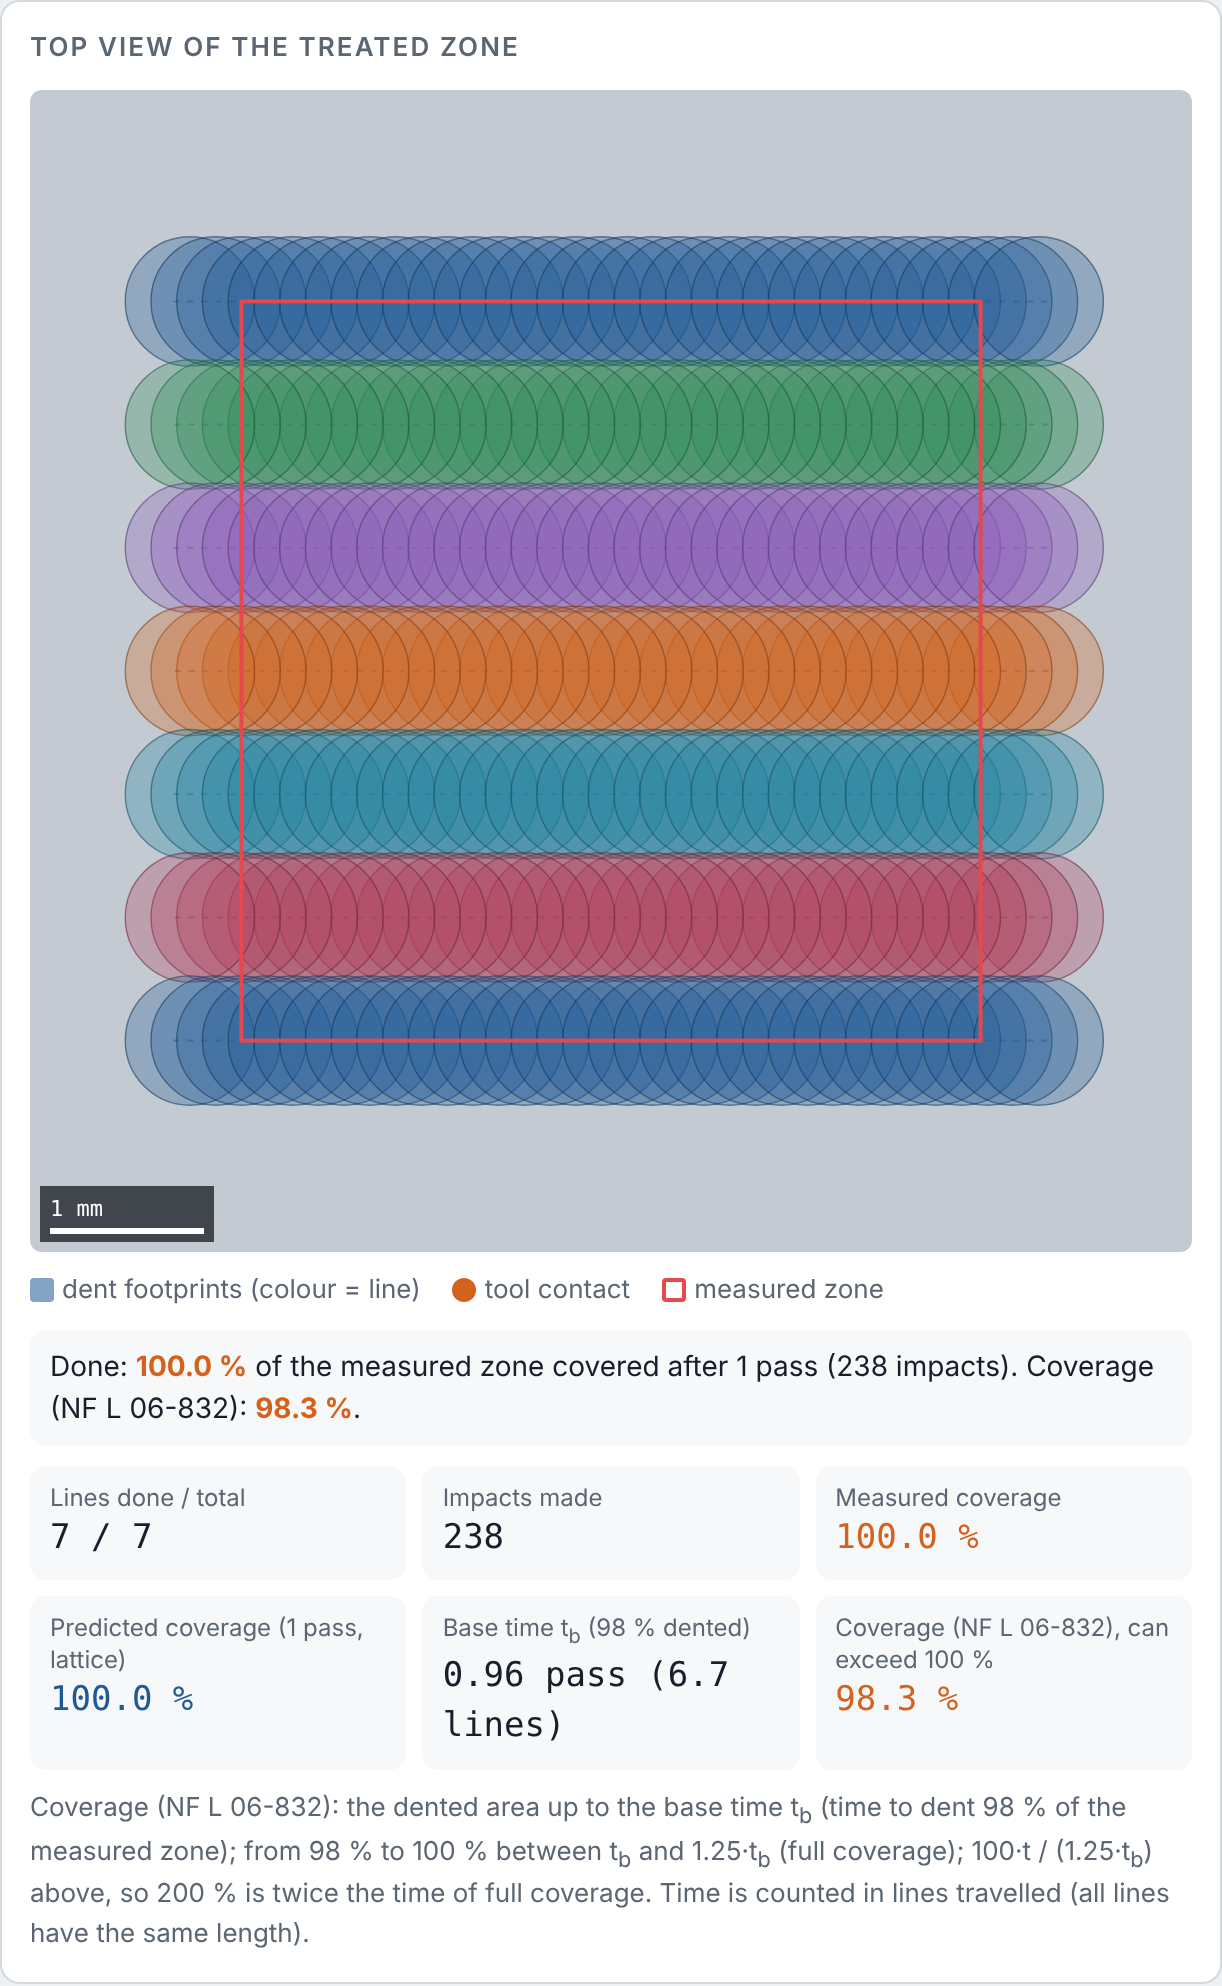
\includegraphics[width=\linewidth]{img/sec0.png}\caption{Top view.}\end{subfigure}\hfill
\begin{subfigure}{0.48\linewidth}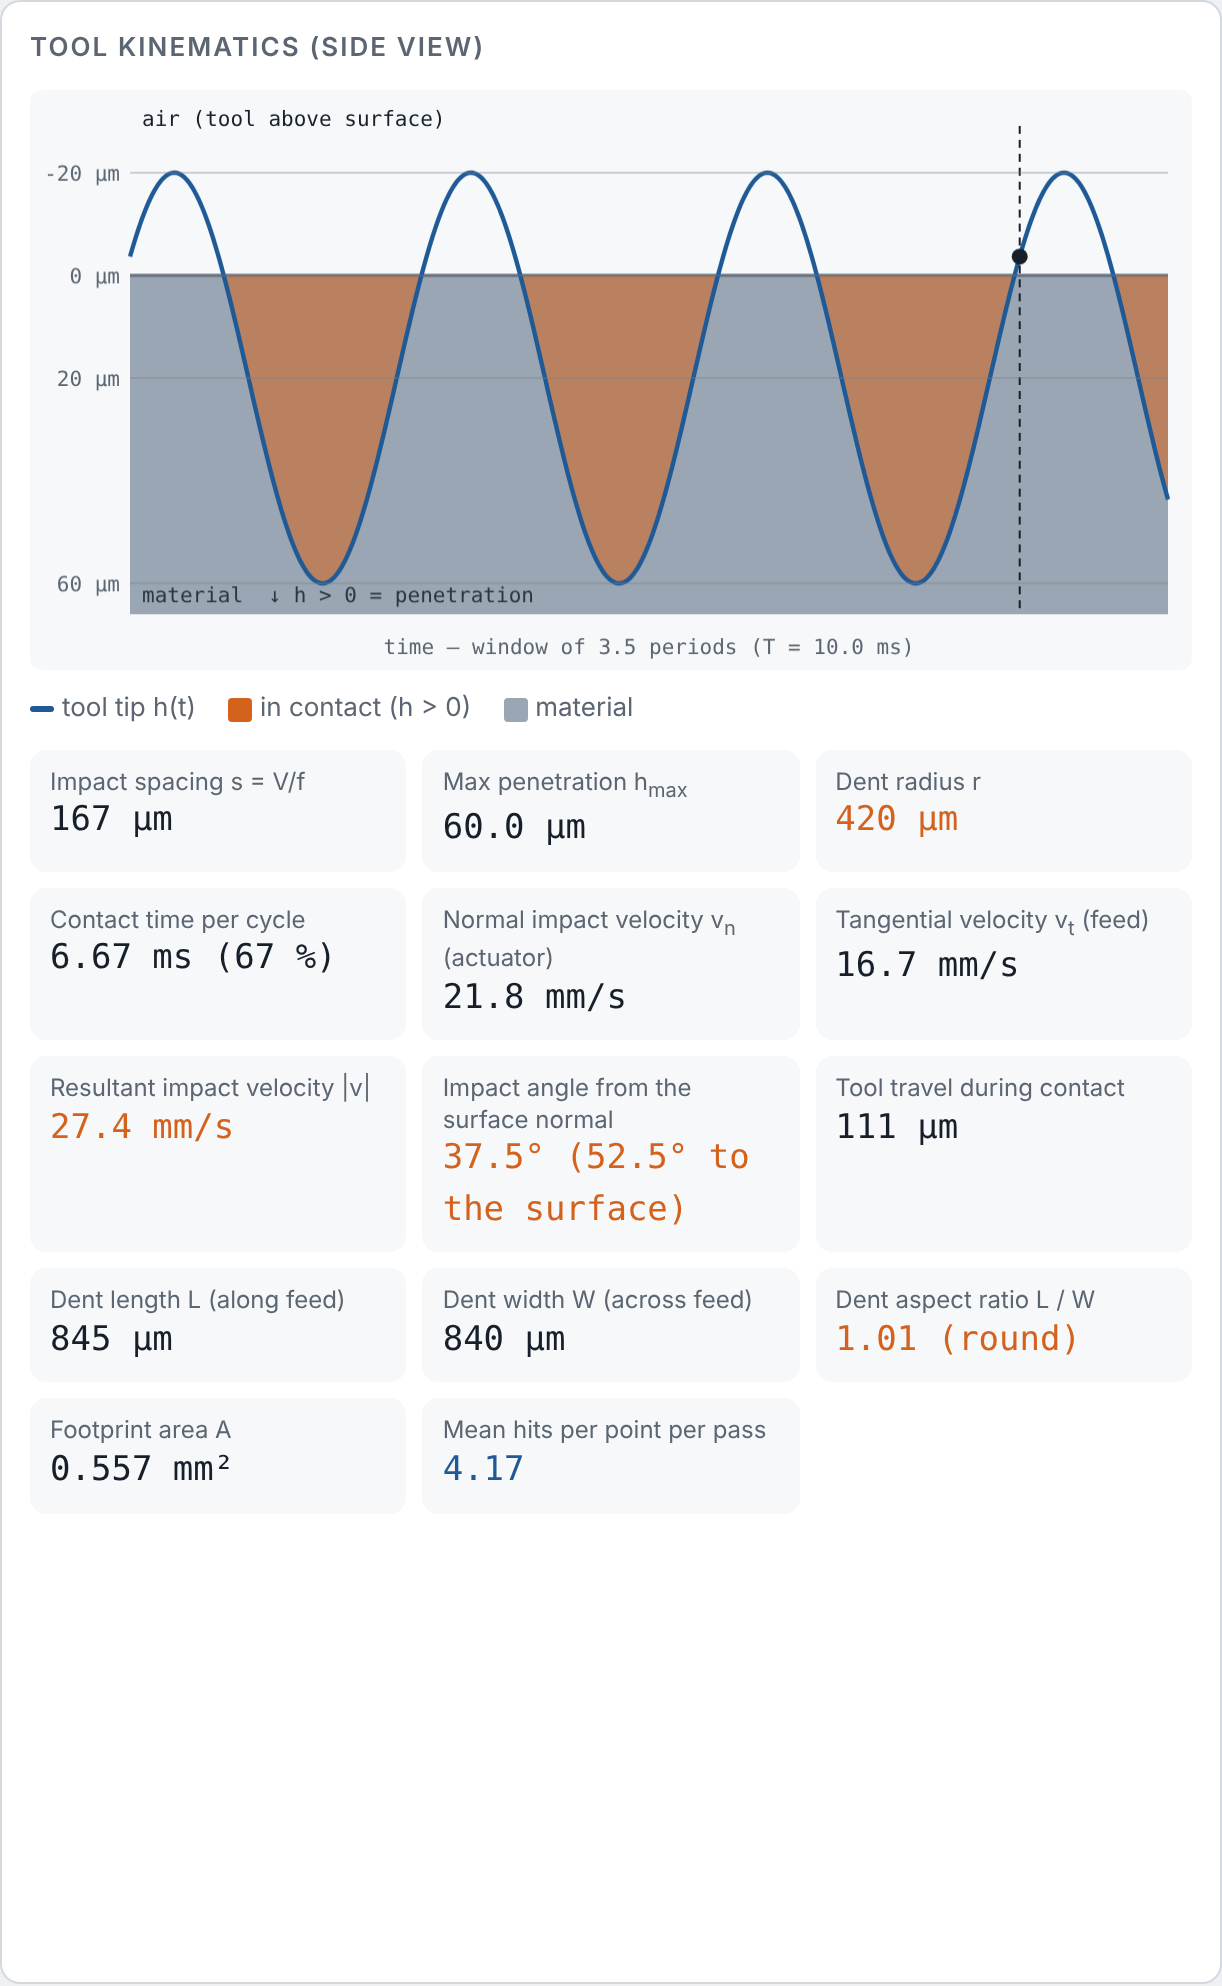
\includegraphics[width=\linewidth]{img/sec1.png}\caption{Tool kinematics.}\end{subfigure}
\caption{The first two panels with the default values.}
\end{figure}

\section{Motion of the tool}\label{sec:kin}

\paragraph{Height of the tool tip.} The sign convention is that $h>0$ means the tool tip is \emph{below} the initial surface, inside the material. The actuator makes the tip oscillate around a median line $U_\mathrm{off}$:
\begin{equation}
h(t)=\eta\,\bigl(U_\mathrm{off}+a\sin(2\pi f t)\bigr),
\end{equation}
where $a$ is the amplitude and $\eta\le1$ a \emph{penetration efficiency}: it accounts in a simple way for the part of the motion lost in the compliance of the machine and of the tool and in the elastic deflection of the part. With $\eta=1$ the tool enters the material by the full stroke. The maximum penetration is
\begin{equation}
h_\mathrm{max}=\eta\,(U_\mathrm{off}+a)\qquad(\SI{60}{\micro m}\text{ with the defaults}).
\end{equation}

\paragraph{Three regimes.}
\begin{itemize}[leftmargin=*]
\item $U_\mathrm{off}+a\le0$: the tool never reaches the surface, \textbf{no contact} (warning on the page).
\item $U_\mathrm{off}-a\ge0$: the tool never leaves the material, the \textbf{contact is continuous} and it ploughs a groove; there are no separate impacts.
\item otherwise, \textbf{impacts}: contact starts at the phase $\theta_1=\arcsin(-U_\mathrm{off}/a)$ and ends at $\theta_2=\pi-\theta_1$.
\end{itemize}

\paragraph{Contact time and velocities.} For impacts, the contact lasts
\begin{equation}
t_c=\frac{\theta_2-\theta_1}{2\pi f}\qquad(\SI{6.67}{ms},\ \text{i.e.\ }67\,\%\text{ of the period}).
\end{equation}
The normal velocity at first contact is the actuator velocity when the tip crosses the surface:
\begin{equation}
v_n=2\pi f\sqrt{a^2-U_\mathrm{off}^2}\qquad(\SI{21.8}{mm/s}),
\end{equation}
and the tangential velocity is the feed, $v_t=V$ (\SI{16.7}{mm/s}). The resultant velocity is $|v|=\sqrt{v_n^2+v_t^2}$ (\SI{27.4}{mm/s}) and its angle from the surface normal is $\arctan(v_t/v_n)$ (37.5°, i.e.\ 52.5° to the surface). During the contact the tool travels $V t_c$ (\SI{111}{\micro m}) along the line.

\section{One dent}\label{sec:dent}

\paragraph{Radius.} A rigid sphere of radius $R=D/2$ pressed to a depth $h$ leaves a circular contact of radius
\begin{equation}
r(h)=\sqrt{2Rh-h^2},\qquad r=r(h_\mathrm{max})=\SI{420}{\micro m}.
\end{equation}
When $h_\mathrm{max}>R$ the radius is capped at $R$ (warning on the page).

\paragraph{Footprint.} Because the tool moves during the contact, the footprint is the union of the contact circles of radius $r(h(t))$ centred at $V(t-t_\mathrm{peak})$, where $t_\mathrm{peak}$ is the time of maximum penetration. The page samples this union and gives:
\begin{itemize}[nosep]
\item the width across the feed $W=2r$ (\SI{840}{\micro m});
\item the length along the feed $L=2\max_t\bigl(|V(t-t_\mathrm{peak})|+r(h(t))\bigr)$ (\SI{845}{\micro m});
\item the aspect ratio $L/W$: below 1.05 ``round'', below 1.2 ``slightly oval'', above ``elongated'';
\item the area $A$ of the footprint (\SI{0.557}{mm^2}).
\end{itemize}
Elongated dents appear when the tool travels a distance comparable to $r$ during the contact (high $V$, large $U_\mathrm{off}$, low $f$). The page then warns that real dents will also show ploughing and a front lip, which the model does not include.

\section{The lattice of impacts}\label{sec:lattice}

\paragraph{Along a line.} Impacts follow one another every
\begin{equation}
s=\frac{V}{f}\qquad(\SI{167}{\micro m}).
\end{equation}

\paragraph{Across the lines.} The lines are spaced by the step-over $p$. The \textbf{phase shift} $\varphi$ moves the impacts of line $j$ by $j\,\frac{\varphi}{360°}\,s$ along the feed: $\varphi=0$ aligns the impacts in columns, $\varphi=180°$ staggers them.

\paragraph{Tool path.} \ui{Zigzag} travels the lines back and forth, \ui{One way} always in the same direction. The footprint is symmetric, so the dents are the same; only the order of the impacts changes.

\paragraph{Passes.} The zone can be treated $N$ times (1 to 10). With \ui{Offset between passes = Half pitch}, every other pass is shifted by $p/2$ across and $s/2$ along the feed, so its dents fall in the gaps of the previous pass.

\paragraph{Measured zone.} The page treats a zone large enough to contain several lines: its height is $L_y=\min(\max(6p,4r),12r)$; lines start and end outside it, so that edge effects are excluded. Coverage and statistics are computed inside the red frame only.

\section{Hits per point and coverage}\label{sec:hits}

\paragraph{Mean number of hits.} One dent of area $A$ is made per cell of area $s\times p$, so the mean number of hits per point and per pass is
\begin{equation}
\lambda=\frac{A}{s\,p}\qquad(4.17).
\end{equation}
After $N$ passes the mean is $N\lambda$. This is the same quantity as $\lambda$ in shot peening, but here the hits are \emph{ordered}: the number of hits varies only between 2 and 6 with the defaults.

\paragraph{When is the surface fully covered?} With aligned lines ($\varphi=0$), the farthest point from the four neighbouring dents is the centre of a cell, at distance $\sqrt{(p/2)^2+(s/2)^2}$. With circular dents the surface is covered in one pass when
\begin{equation}
\Bigl(\frac p2\Bigr)^2+\Bigl(\frac s2\Bigr)^2\le r^2
\quad\Longleftrightarrow\quad p\le 2\sqrt{r^2-(s/2)^2}\qquad(p\le\SI{823}{\micro m}).
\end{equation}
Staggered lines ($\varphi=180°$) tolerate a slightly larger step-over.

\paragraph{Readouts.}
\begin{itemize}[nosep]
\item \ui{Measured coverage}: share of the measured zone with at least one dent (pixel count on the grid).
\item \ui{Predicted coverage (1 pass, lattice)}: the same quantity computed on one periodic cell $s\times p$ of the lattice.
\item \ui{Mean hits per point}, \ui{Min / max hits}, \ui{Never-hit surface}.
\item \ui{Treatment rate}: $Vp$ (\SI{13.4}{mm^2/s}); time to treat \SI{1}{cm^2}: $100/(Vp)$ (\SI{7.5}{s}).
\end{itemize}

\begin{figure}[H]
\centering
\begin{subfigure}{0.48\linewidth}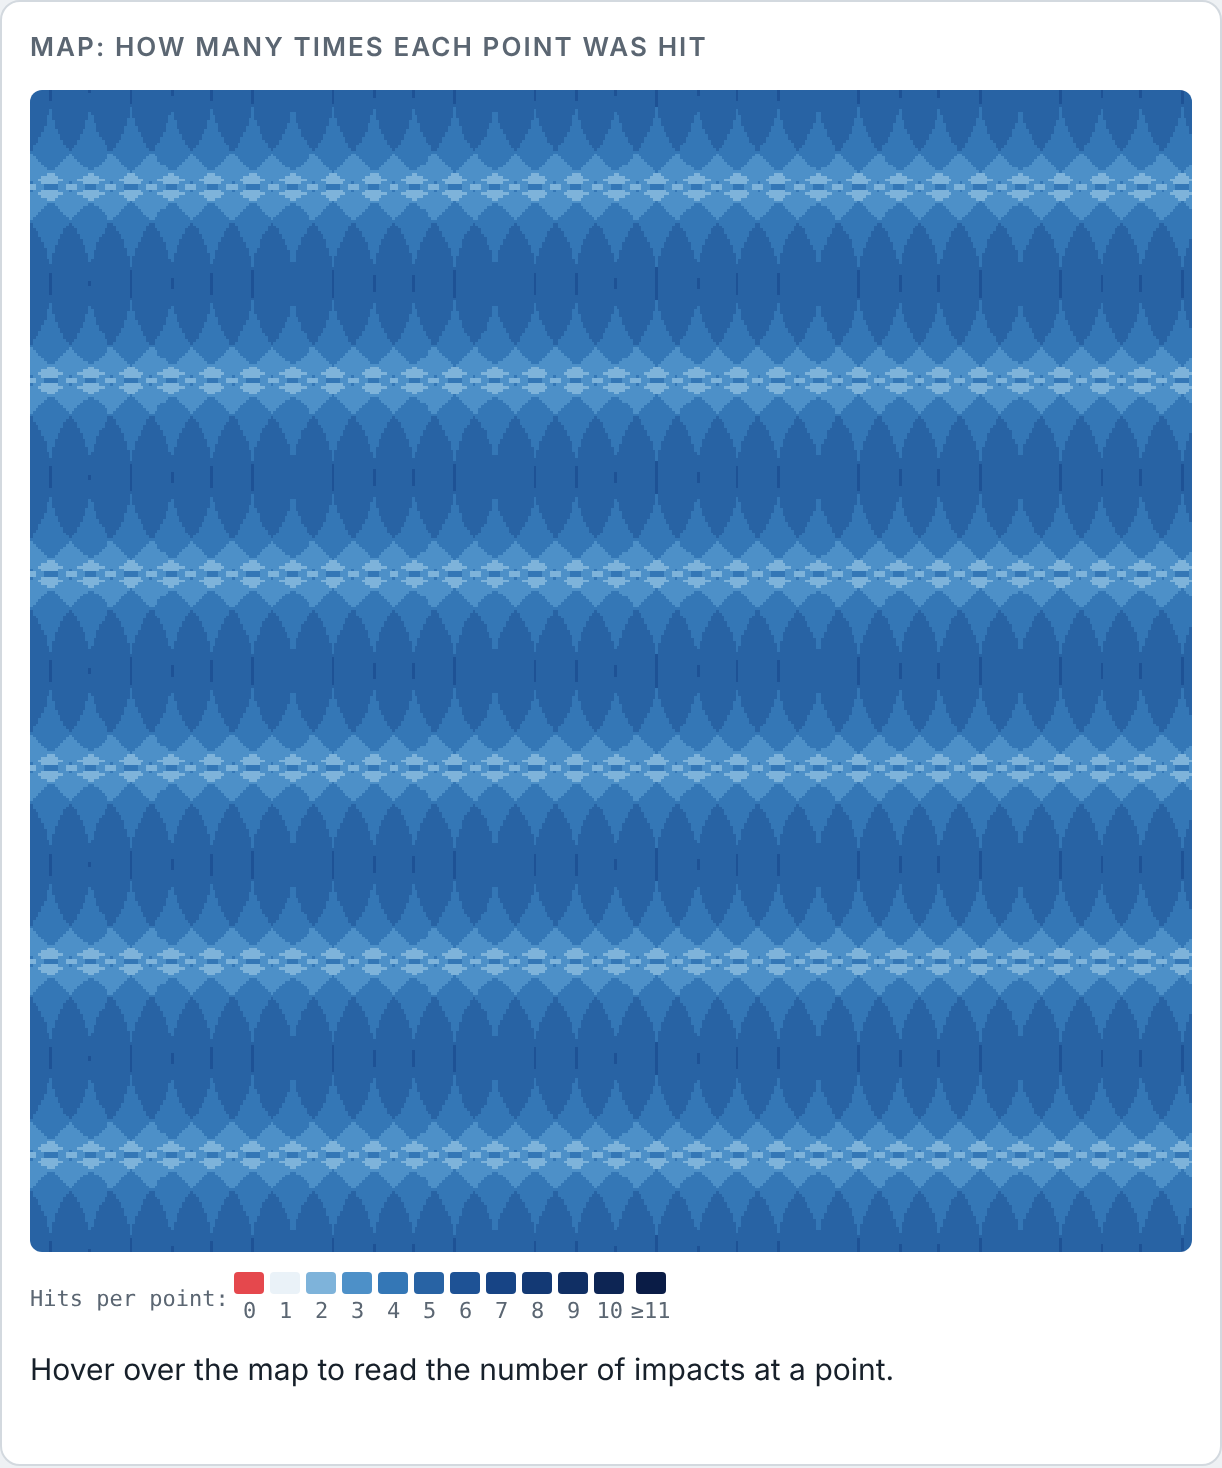
\includegraphics[width=\linewidth]{img/sec2.png}\caption{Hit map.}\end{subfigure}\hfill
\begin{subfigure}{0.48\linewidth}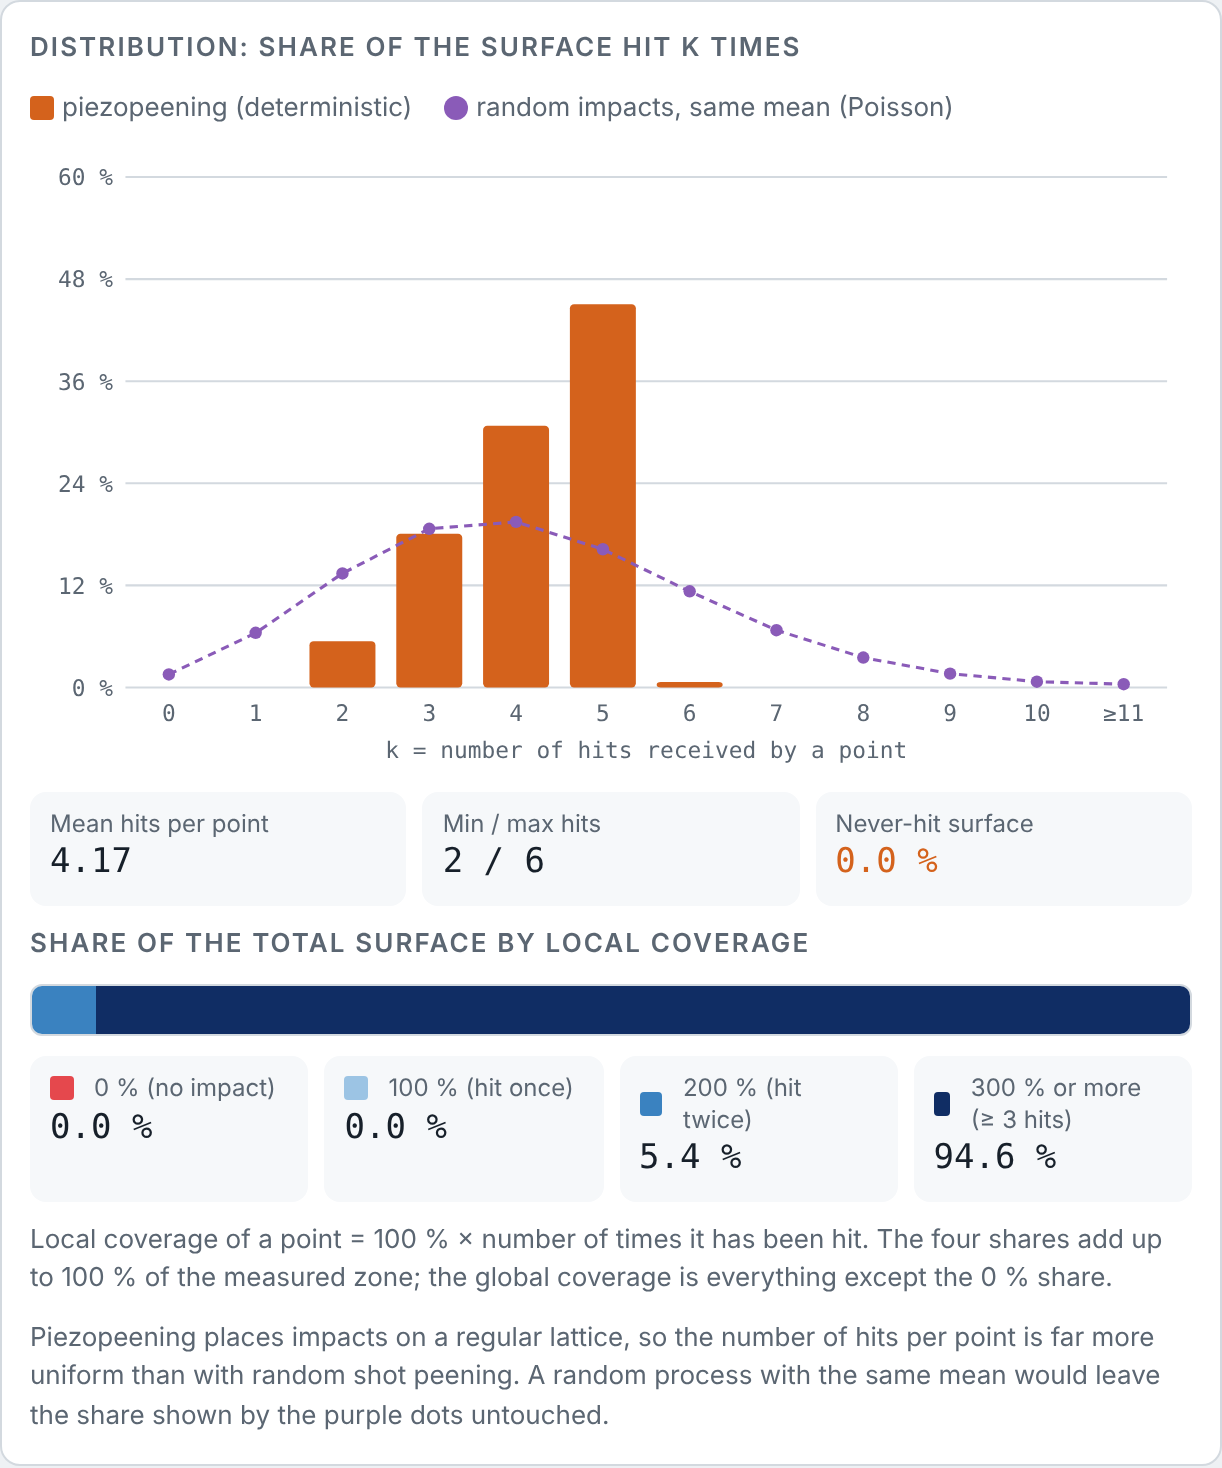
\includegraphics[width=\linewidth]{img/sec3.png}\caption{Distribution of hits.}\end{subfigure}
\caption{Number of hits per point. The bars are the piezopeening lattice, the purple dots the Poisson law with the same mean.}
\end{figure}

\paragraph{Distribution and share by local coverage.} The bar chart gives the share of the surface hit $k$ times. The coloured bar below groups it as the page's ``local coverage'' convention: 0\,\% (never hit), 100\,\% (hit once), 200\,\% (hit twice), 300\,\% or more. With the defaults: 0, 0, 5.4 and 94.6\,\%. The four shares add up to 100\,\% of the zone; the global coverage is everything except the 0\,\% share.

\section{Coverage above 100\,\% (NF~L~06-832)}\label{sec:nf}

NF~L~06-832 defines the \textbf{base time} $t_b$ as the time needed to dent 98\,\% of the surface, \textbf{full coverage (100\,\%)} as $1.25\,t_b$, and a coverage of $C$\,\% as $\frac{C}{100}\times1.25\,t_b$. On the page, the time is counted in lines travelled (all lines have the same length): the dented share of the measured zone is recorded after each line, and $t_b$ is the moment it reaches 98\,\%, interpolated linearly within the line since the dents are laid one after the other. The readout \ui{Base time $t_b$} gives it in passes and in lines (0.96 pass, 6.7 lines with the defaults); it reads ``not reached'' when the planned passes never dent 98\,\% of the zone.

\paragraph{The readout \ui{Coverage (NF L 06-832)}.} Coverage is the dented area divided by the total area as long as it can be measured, i.e.\ up to 98\,\%. Beyond, NF~L~06-832 counts time. The page combines both in one value, $C(t)$, continuous and increasing:
\begin{equation}
C(t)=\begin{cases}
\text{dented area (\%)} & t\le t_b\quad(\text{reaches }98\,\%\text{ at }t_b)\\[2pt]
98+2\,\dfrac{t/t_b-1}{0.25} & t_b<t\le1.25\,t_b\quad(98\to100\,\%)\\[6pt]
100\,\dfrac{t}{1.25\,t_b} & t>1.25\,t_b
\end{cases}
\end{equation}
With the option \ui{Full coverage (100\,\%) = base time}, the middle interval disappears: $C=100\,t/t_b$ after the base time. The number of passes (or the time) for a specified coverage $C$ is the inverse of this function: below 98\,\% it comes from the dented area, above 100\,\% it is $\frac{C}{100}\times1.25\,t_b$.

\begin{center}\small
\begin{tabular}{@{}lccccccc@{}}
\toprule
Passes $n$ (reference case, $K=0.337$) & 1 & 3 & 6 & 11.6 ($t_b$) & 13.0 & 14.5 & 29.0\\ \midrule
Dented area (\%) & 28.6 & 63.6 & 86.8 & 98.0 & 98.8 & 99.25 & 99.99\\
Coverage (NF L 06-832) (\%) & 28.6 & 63.6 & 86.8 & 98 & 99 & 100 & 200\\ \bottomrule
\end{tabular}
\end{center}

\paragraph{Local coverage of a point.} On the flat-part and cylinder simulators the same rule is applied to each point, with time replaced by the number of impacts it has received (proportional to time on an even treatment): $C(x,y)=1-e^{-\lambda}$ up to $\lambda=\ln50=3.91$ (98\,\%), then 98 to 100\,\% up to $\lambda=1.25\ln50=4.89$, and $100\,\lambda/4.89$ above. The hover readout gives it, and the map can show it (\ui{Map shows: coverage NF L 06-832}).


\noindent The table above is for random shot peening; for piezopeening the dented area rises almost linearly with time, line after line, until the lattice closes. Examples:
\begin{itemize}[nosep]
\item defaults: $t_b=0.96$ pass; after 1 pass the zone is 100\,\% dented and $C=98.3\,\%$; 3 passes give $C=249\,\%$;
\item $p=\SI{1.2}{mm}$, 1 to 4 passes on the same path: the gaps are never filled, 98\,\% is not reached and $C$ stays at the dented area, 71.1\,\%;
\item $p=\SI{1.2}{mm}$ with \ui{Half pitch}: $t_b=1.74$ passes; 2 passes give $C=99.2\,\%$, 4 passes 183\,\%.
\end{itemize}
With the option \ui{Full coverage (100\,\%) = base time}, 3 passes with the defaults give 311\,\%.

\section{Depth and waviness}\label{sec:depth}

\paragraph{Depth map.} Each point keeps the deepest trace of the sphere over all impacts:
\begin{equation}
z(x,y)=\max_\text{impacts}\Bigl[h-\bigl(R-\sqrt{R^2-d^2}\bigr)\Bigr]^+,
\end{equation}
where $d$ is the distance from the point to the axis of the tool at that moment, and $h$ its penetration. The colour scale goes from 0 to $h_\mathrm{max}$; untreated points are grey. Hovering gives the depth; clicking moves both profile lines to that point; the sliders move them separately, and \ui{Snap horizontal line to nearest tool path} puts the horizontal line on a line of impacts.

\paragraph{Profiles.} The vertical line gives the profile across the feed (scallops between lines), the horizontal line the profile along the feed (scallops between impacts).

\paragraph{Readouts.} Max depth in the measured zone (60.0\,µm), mean depth (41.2\,µm), shallowest point (4.8\,µm), peak-to-valley of the treated surface (55.1\,µm), and the theoretical ridge height between two neighbouring traces at a spacing $e$:
\begin{equation}
H(e)=R-\sqrt{R^2-(e/2)^2},
\end{equation}
with $e=p$ across the feed (\SI{54.3}{\micro m}) and $e=s$ along it (\SI{2.3}{\micro m}). The ridge cannot exceed $h_\mathrm{max}$; when $H(p)>h_\mathrm{max}$, a strip of untouched material remains between the lines. The kinematic model neglects the tool travel during contact for this formula, elastic recovery and pile-up.

\begin{figure}[H]
\centering
\begin{subfigure}{0.48\linewidth}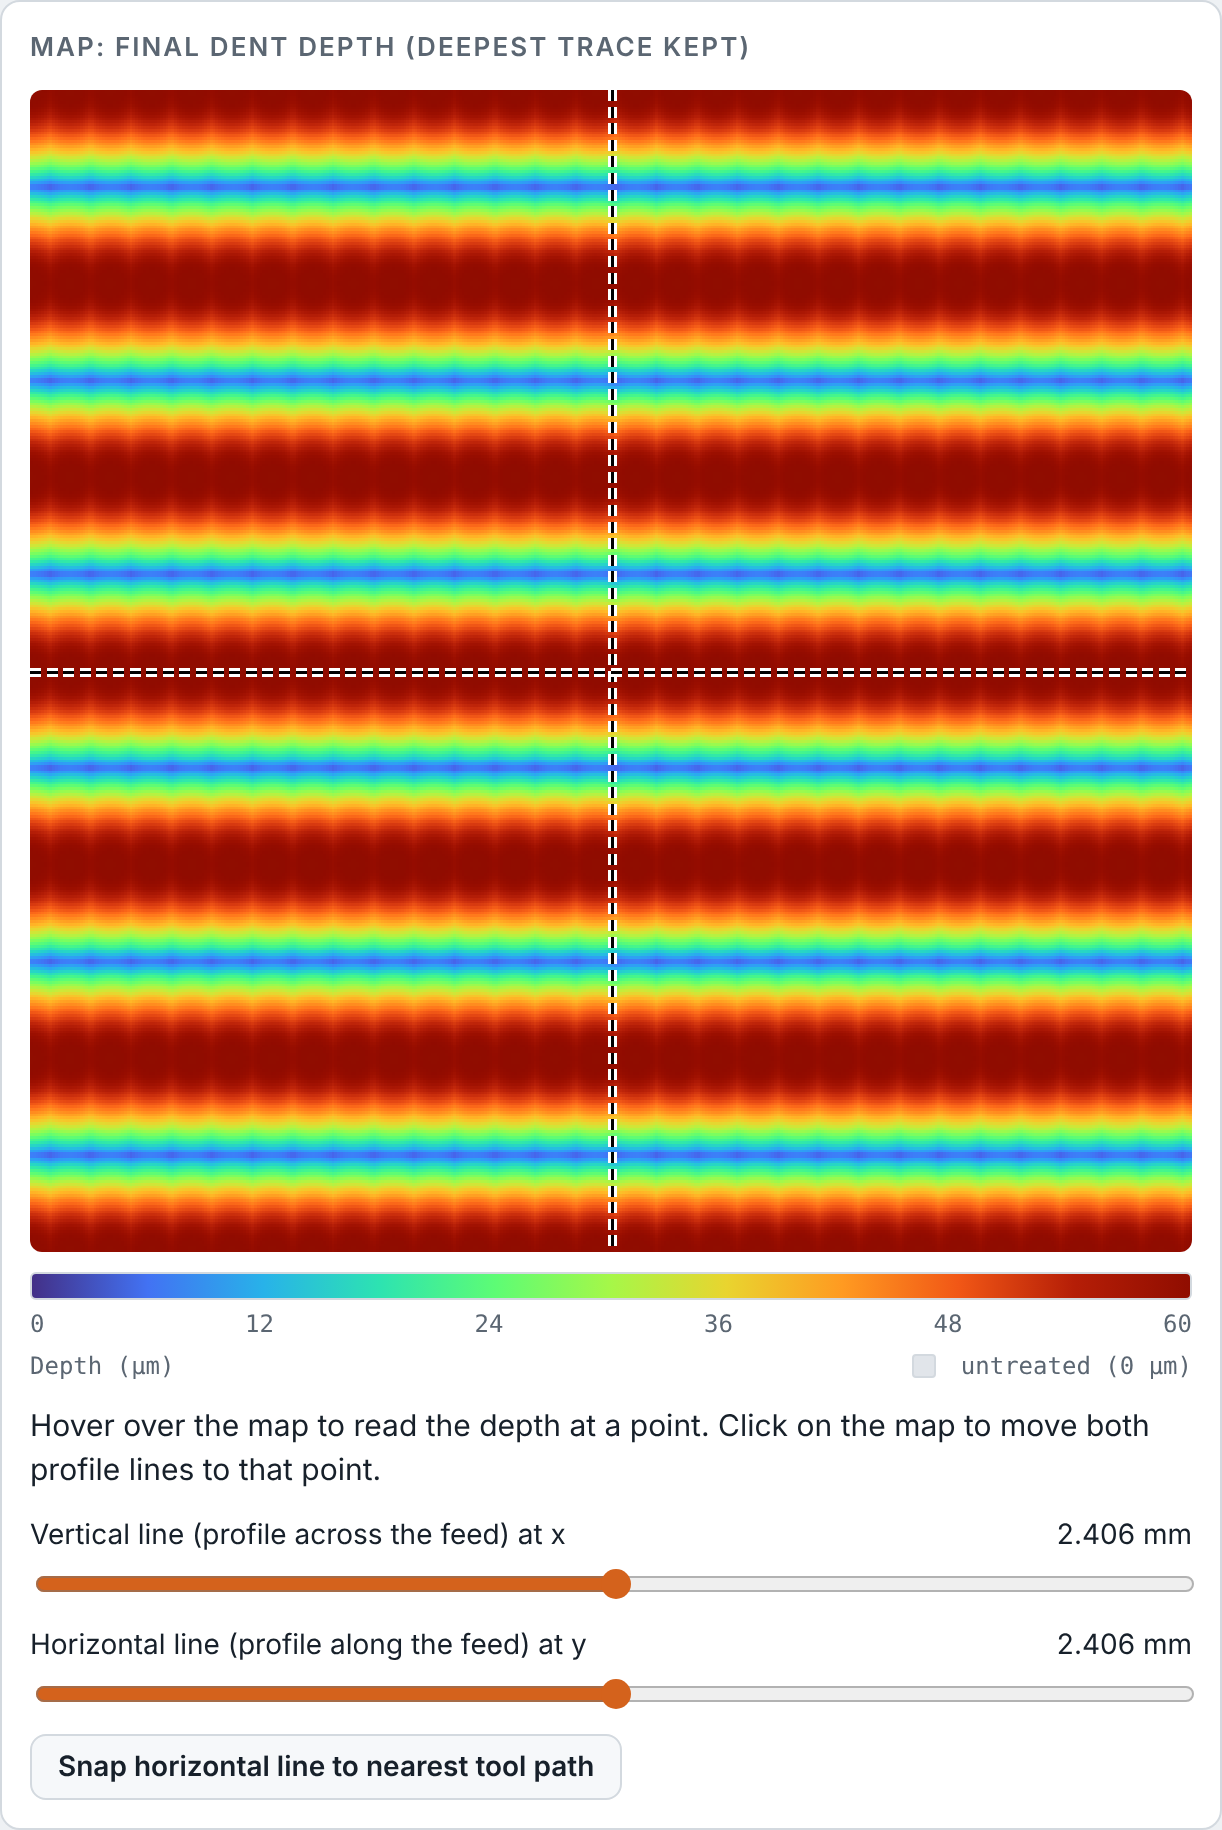
\includegraphics[width=\linewidth]{img/sec4.png}\caption{Depth map.}\end{subfigure}\hfill
\begin{subfigure}{0.48\linewidth}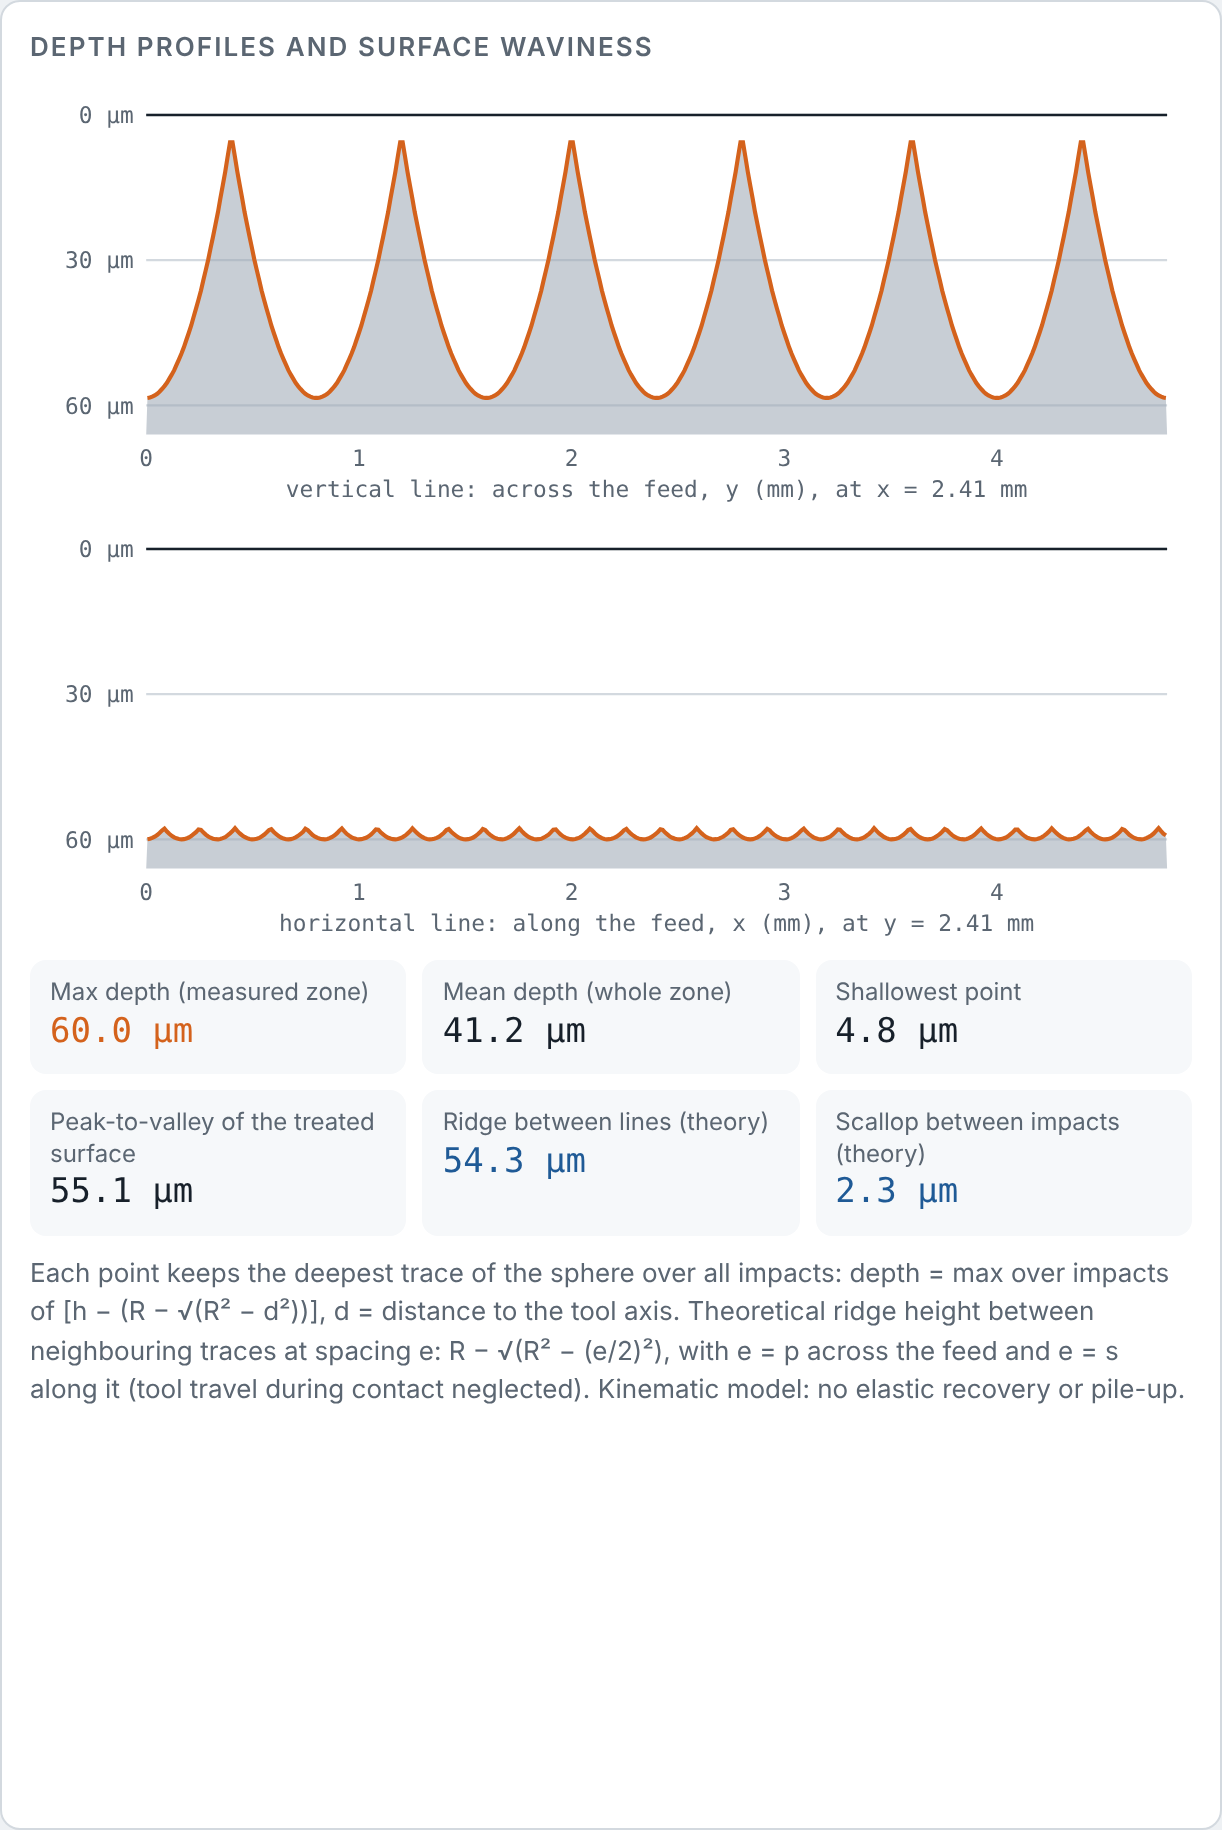
\includegraphics[width=\linewidth]{img/sec5.png}\caption{Profiles and waviness.}\end{subfigure}
\caption{Depth with the defaults: deep grooves along the lines (54\,µm ridges), almost flat along the feed (2.3\,µm scallops).}
\end{figure}

\section{Roughness}\label{sec:rough}

The depth map gives the height of the treated surface at every point of the grid, $z=-\text{depth}$, measured from the initial surface. The page computes from it the usual roughness parameters, in two tables.

\paragraph{2D roughness (ISO 4287).} Each profile $z(u)$, $u$ along the profile, is referred to its mean line ($\bar z=0$). With $n$ points:
\begin{gather}
R_a=\frac1n\sum|z_i|,\qquad R_q=\sqrt{\frac1n\sum z_i^2},\qquad R_{sk}=\frac{1}{nR_q^3}\sum z_i^3,\qquad R_{ku}=\frac{1}{nR_q^4}\sum z_i^4,\\
R_p=\max z_i,\qquad R_v=-\min z_i,\qquad R_t=R_p+R_v,\qquad R_z=\frac15\sum_{k=1}^{5}\bigl(\max_k z-\min_k z\bigr),
\end{gather}
where $\max_k$ and $\min_k$ are taken over the $k$-th of five equal sampling lengths, and $RS_m$ is the mean spacing of the profile elements, measured between successive up-crossings of the mean line. Four columns are given: the profile across the feed at the vertical line $x$, the profile along the feed at the horizontal line $y$ (the two lines of the depth map), and the mean of each parameter over all the parallel profiles of the measured zone, across and along the feed.

\emph{No filter is applied}: the zone is only a few millimetres long, too short for the standard cut-off $\lambda_c=\SI{0.8}{mm}$ and its evaluation length. Strictly these are the primary-profile parameters $P_a$, $P_q$\ldots; they coincide with the $R$ parameters when the waviness is negligible. With a step-over of 0.8~mm, a real measurement filtered at $\lambda_c=\SI{0.8}{mm}$ would remove part of the scallops across the feed.

\paragraph{3D roughness (ISO 25178).} The same definitions over the whole surface of the measured zone, referred to its mean plane: $S_a$, $S_q$, $S_{sk}$, $S_{ku}$, the maximum peak height $S_p$, the maximum pit depth $S_v$, the maximum height $S_z=S_p+S_v$, and two hybrid parameters computed with finite differences on the grid:
\begin{equation}
S_{dq}=\sqrt{\frac1A\iint\Bigl[\Bigl(\frac{\partial z}{\partial x}\Bigr)^2+\Bigl(\frac{\partial z}{\partial y}\Bigr)^2\Bigr]dA},\qquad
S_{dr}=\frac1A\iint\Bigl[\sqrt{1+\Bigl(\frac{\partial z}{\partial x}\Bigr)^2+\Bigl(\frac{\partial z}{\partial y}\Bigr)^2}-1\Bigr]dA .
\end{equation}

\paragraph{Default values.}
\begin{center}\small
\begin{tabular}{@{}lcccc@{\qquad}lc@{}}
\toprule
 & across, line & along, line & across, mean & along, mean & & 3D\\ \midrule
$R_a$ (µm) & 13.90 & 0.60 & 13.89 & 0.61 & $S_a$ (µm) & 13.90\\
$R_q$ (µm) & 16.16 & 0.69 & 16.15 & 0.70 & $S_q$ (µm) & 16.17\\
$R_p$ / $R_v$ (µm) & 34.8 / 18.0 & 1.5 / 0.8 & 34.8 / 18.0 & 1.6 / 0.8 & $S_p$ / $S_v$ (µm) & 36.4 / 18.7\\
$R_t$, $R_z$ (µm) & 52.8, 52.8 & 2.3, 2.3 & 52.8, 52.8 & 2.4, 2.3 & $S_z$ (µm) & 55.1\\
$R_{sk}$ & 0.65 & 0.63 & 0.65 & 0.63 & $S_{sk}$ & 0.65\\
$R_{ku}$ & 2.16 & 2.13 & 2.16 & 2.13 & $S_{ku}$ & 2.16\\
$RS_m$ (mm) & 0.800 & 0.167 & 0.800 & 0.167 & $S_{dq}$; $S_{dr}$ & 0.157; 1.22\,\%\\ \bottomrule
\end{tabular}
\end{center}

\paragraph{Reading the values.} The surface is a regular pattern of spherical scallops. Across the feed the profile is a series of circular arcs of radius $R$ and width $p$, so $RS_m=p$ and $R_t\approx H(p)=\SI{54.3}{\micro m}$; along the feed the arcs have the width $s$, much smaller, so the roughness along the feed is about 20 times lower. For this periodic profile the exact values are $R_a=\SI{13.89}{\micro m}$, $R_q=\SI{16.15}{\micro m}$, $R_{sk}=0.65$ and $R_{ku}=2.16$, as found by the page; $R_t$ is slightly lower on the page (52.8 instead of \SI{54.3}{\micro m}) because the sharp ridges fall between two grid points. The skewness is positive (sharp ridges between rounded valleys) and the kurtosis below 3 (a regular, bounded surface), unlike a random shot-peened surface. Halving the step-over ($p=\SI{0.4}{mm}$) divides $R_a$ across the feed by four (3.43\,µm), since the scallop height varies as $p^2/(8R)$.

\paragraph{Limits.} The model surface is the envelope of rigid sphere traces: no elastic recovery, no pile-up at the edges of the dents, no material flow and no initial roughness. Real values will differ, especially $S_p$, $S_z$ and $S_{ku}$, which are sensitive to pile-up.

\begin{figure}[H]
\centering
\begin{subfigure}{0.48\linewidth}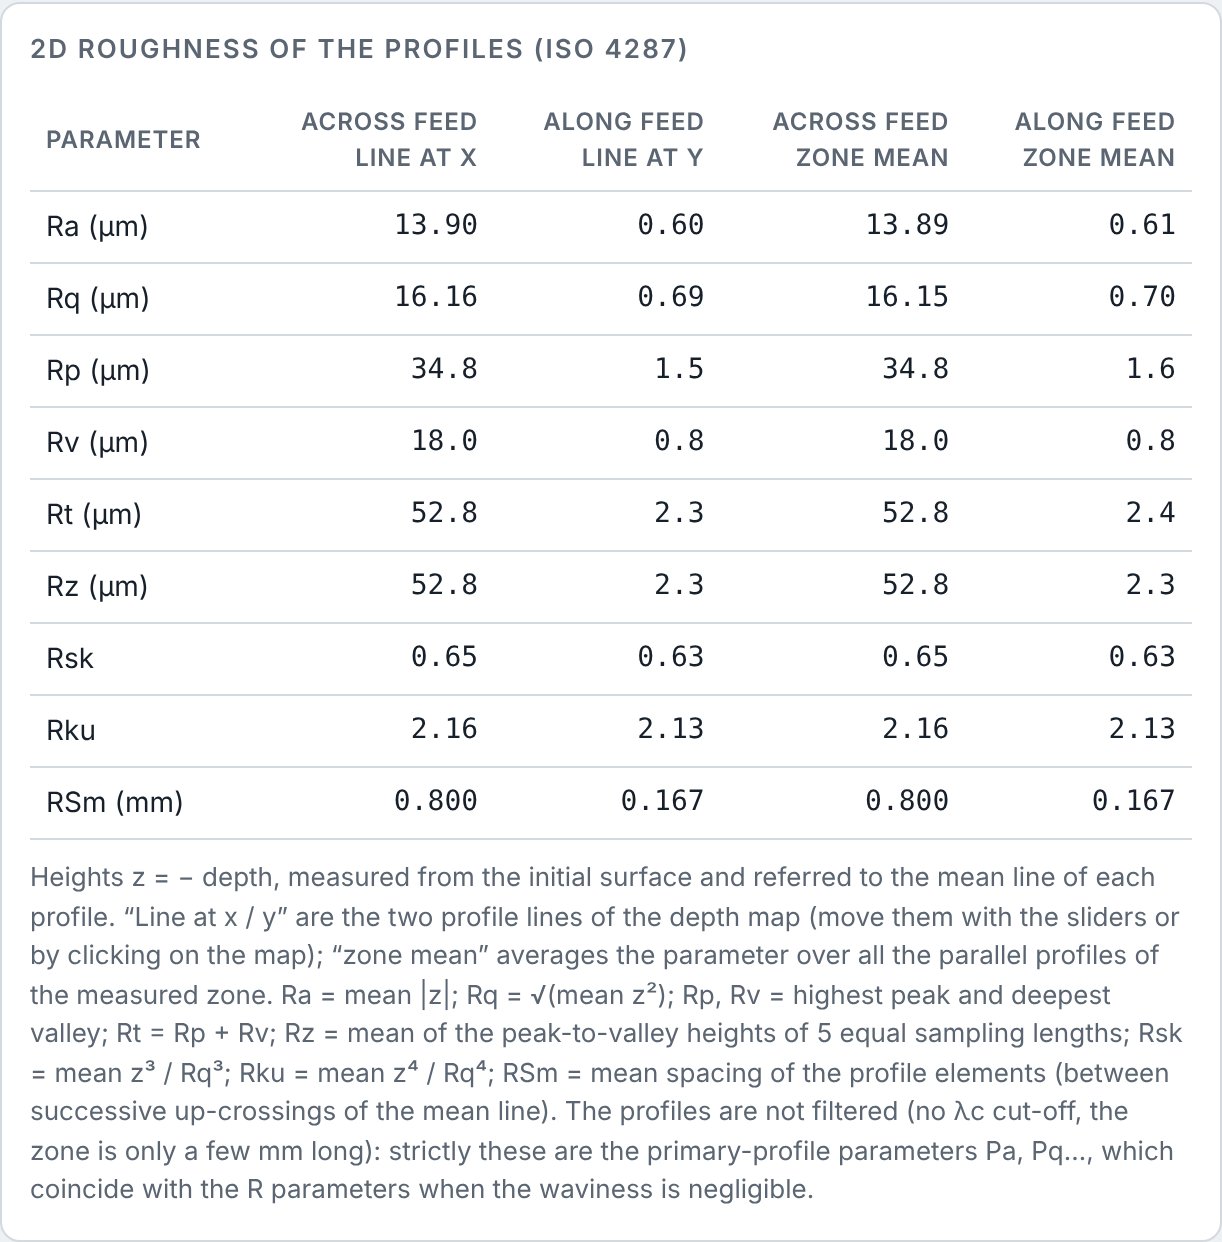
\includegraphics[width=\linewidth]{img/sec6.png}\caption{2D roughness.}\end{subfigure}\hfill
\begin{subfigure}{0.48\linewidth}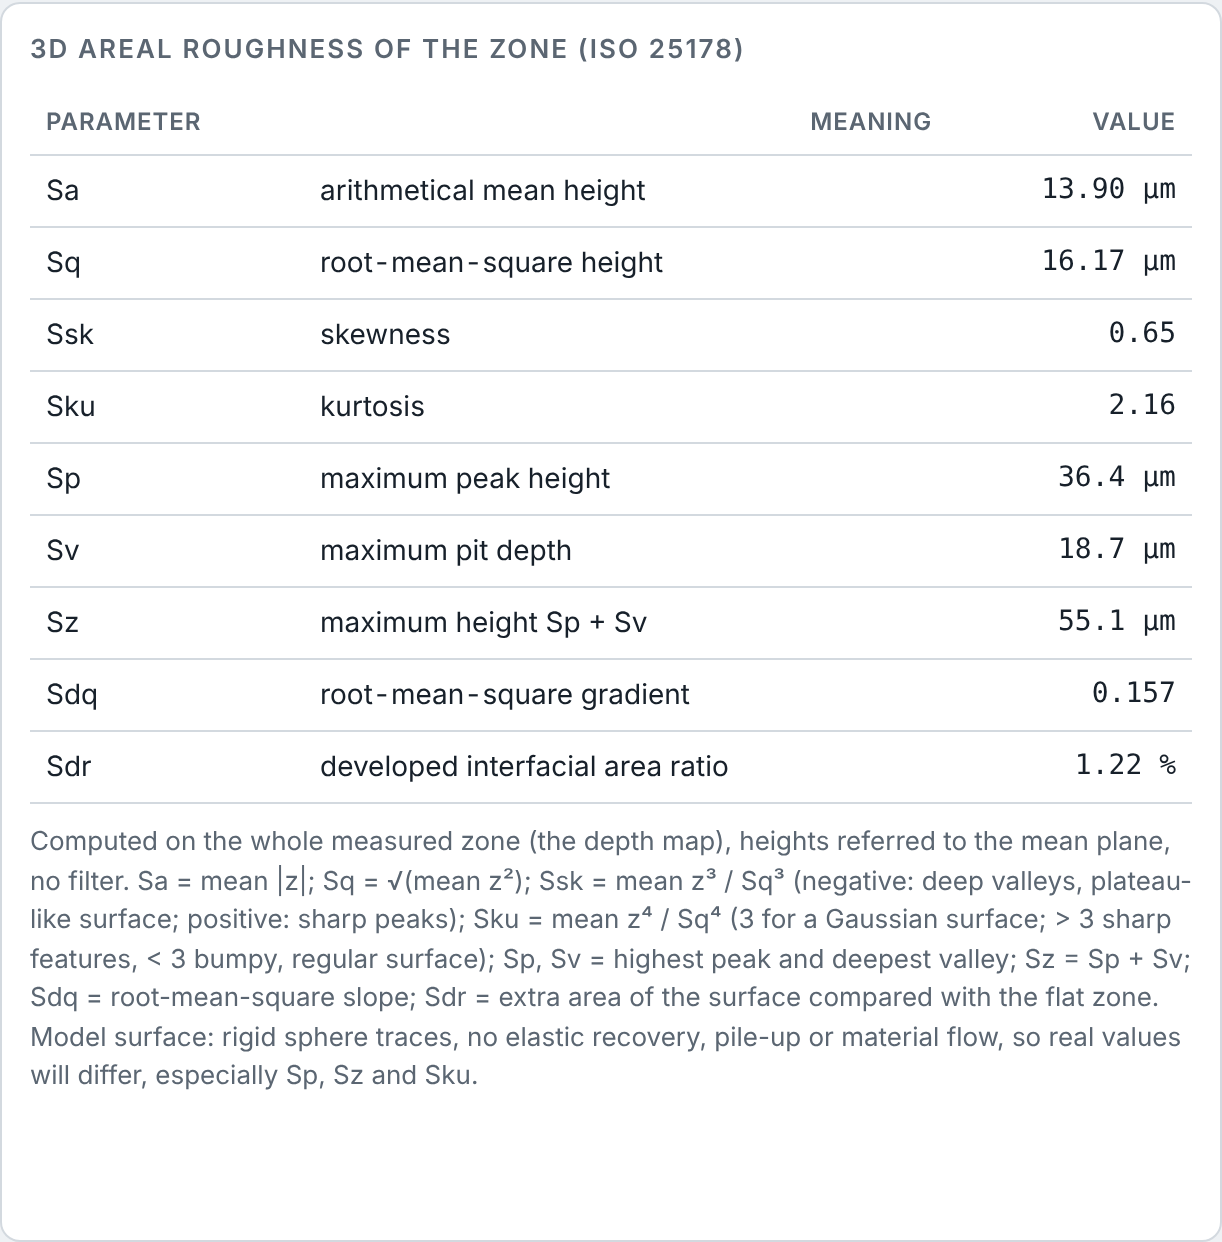
\includegraphics[width=\linewidth]{img/sec7.png}\caption{3D roughness.}\end{subfigure}
\caption{Roughness panels with the default values.}
\end{figure}

\section{Comparison with random impacts}\label{sec:random}

The random map uses the same zone, the same dent shape and the same number of impacts per mm² ($N_\mathrm{imp}$ dents in a zone of area $s\,p$ per dent), but places each dent at a random position, as shot peening does. The number of hits per point then follows the Poisson law
\begin{equation}
P(k)=e^{-\lambda}\frac{\lambda^k}{k!},\qquad \text{untouched share }e^{-\lambda},\qquad\text{standard deviation }\sqrt\lambda .
\end{equation}
With $\lambda=4.17$: about 1.5\,\% untouched and a standard deviation of 2.0, against 0 and 0.92 for the lattice. \ui{New random draw} draws a new set of positions; the column changes slightly from one draw to the next because the zone contains only a few hundred impacts.

\begin{figure}[H]
\centering
\begin{subfigure}{0.48\linewidth}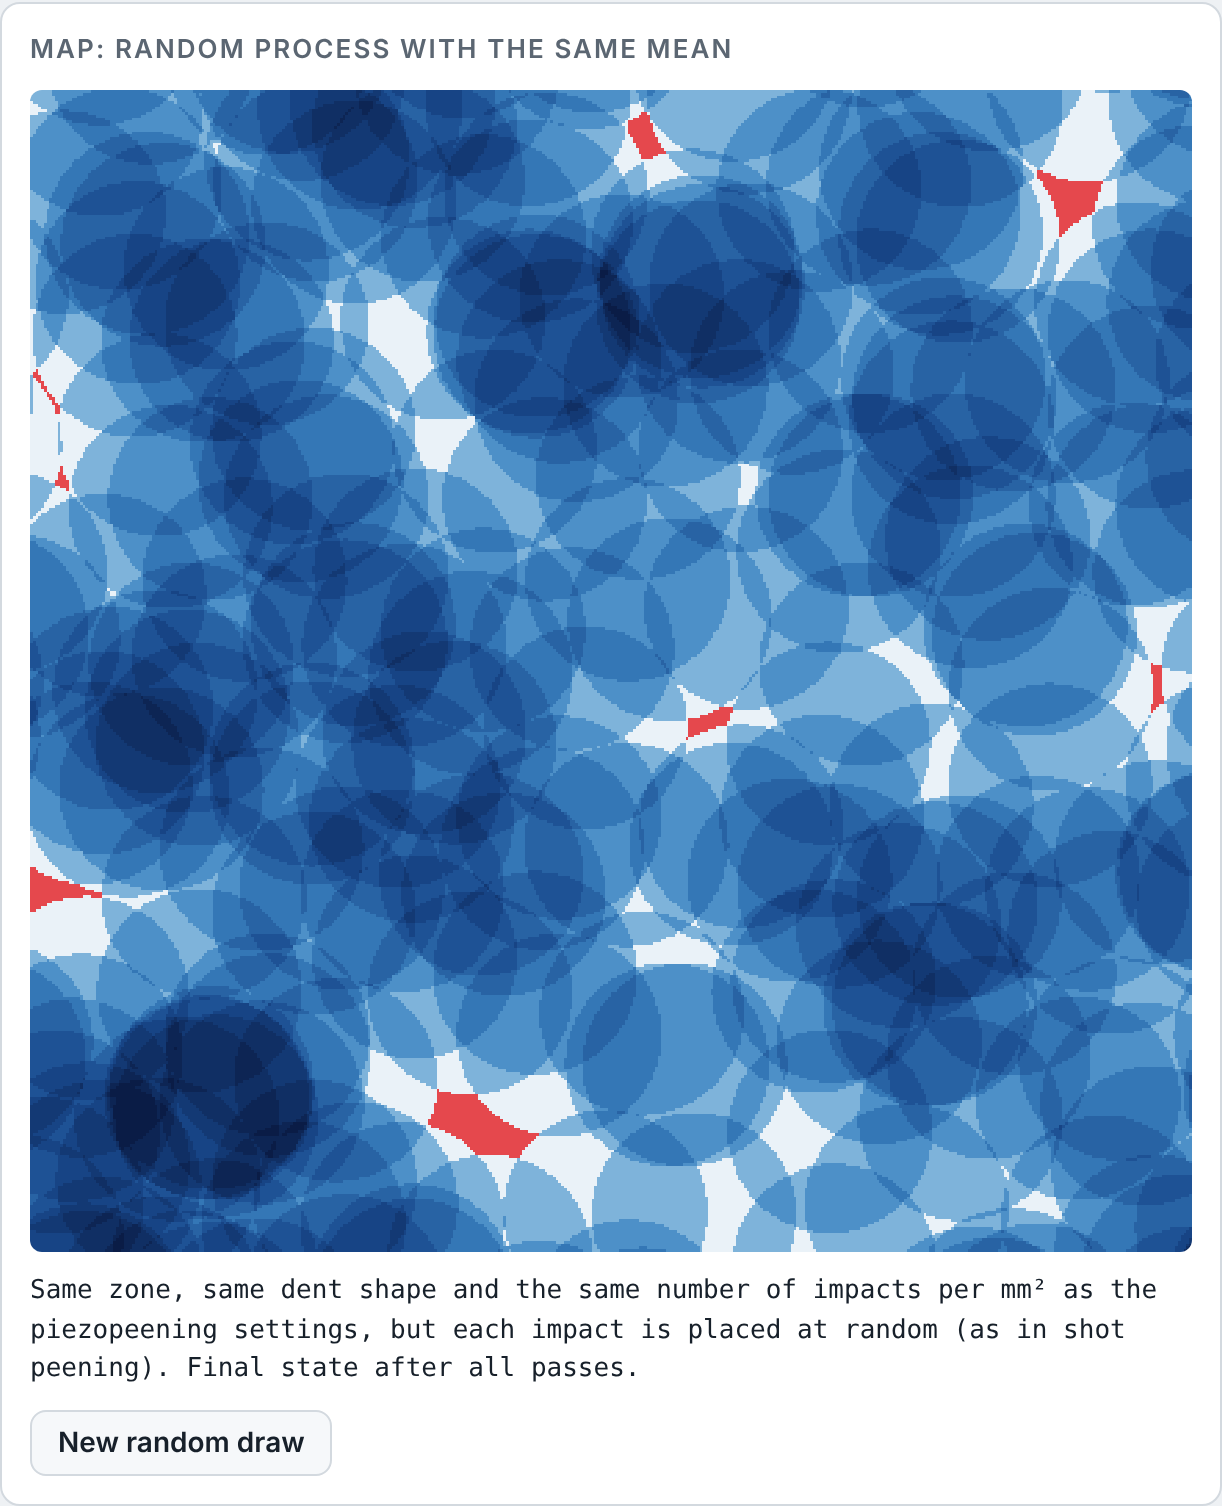
\includegraphics[width=\linewidth]{img/sec8.png}\caption{Random map (red: never hit).}\end{subfigure}\hfill
\begin{subfigure}{0.48\linewidth}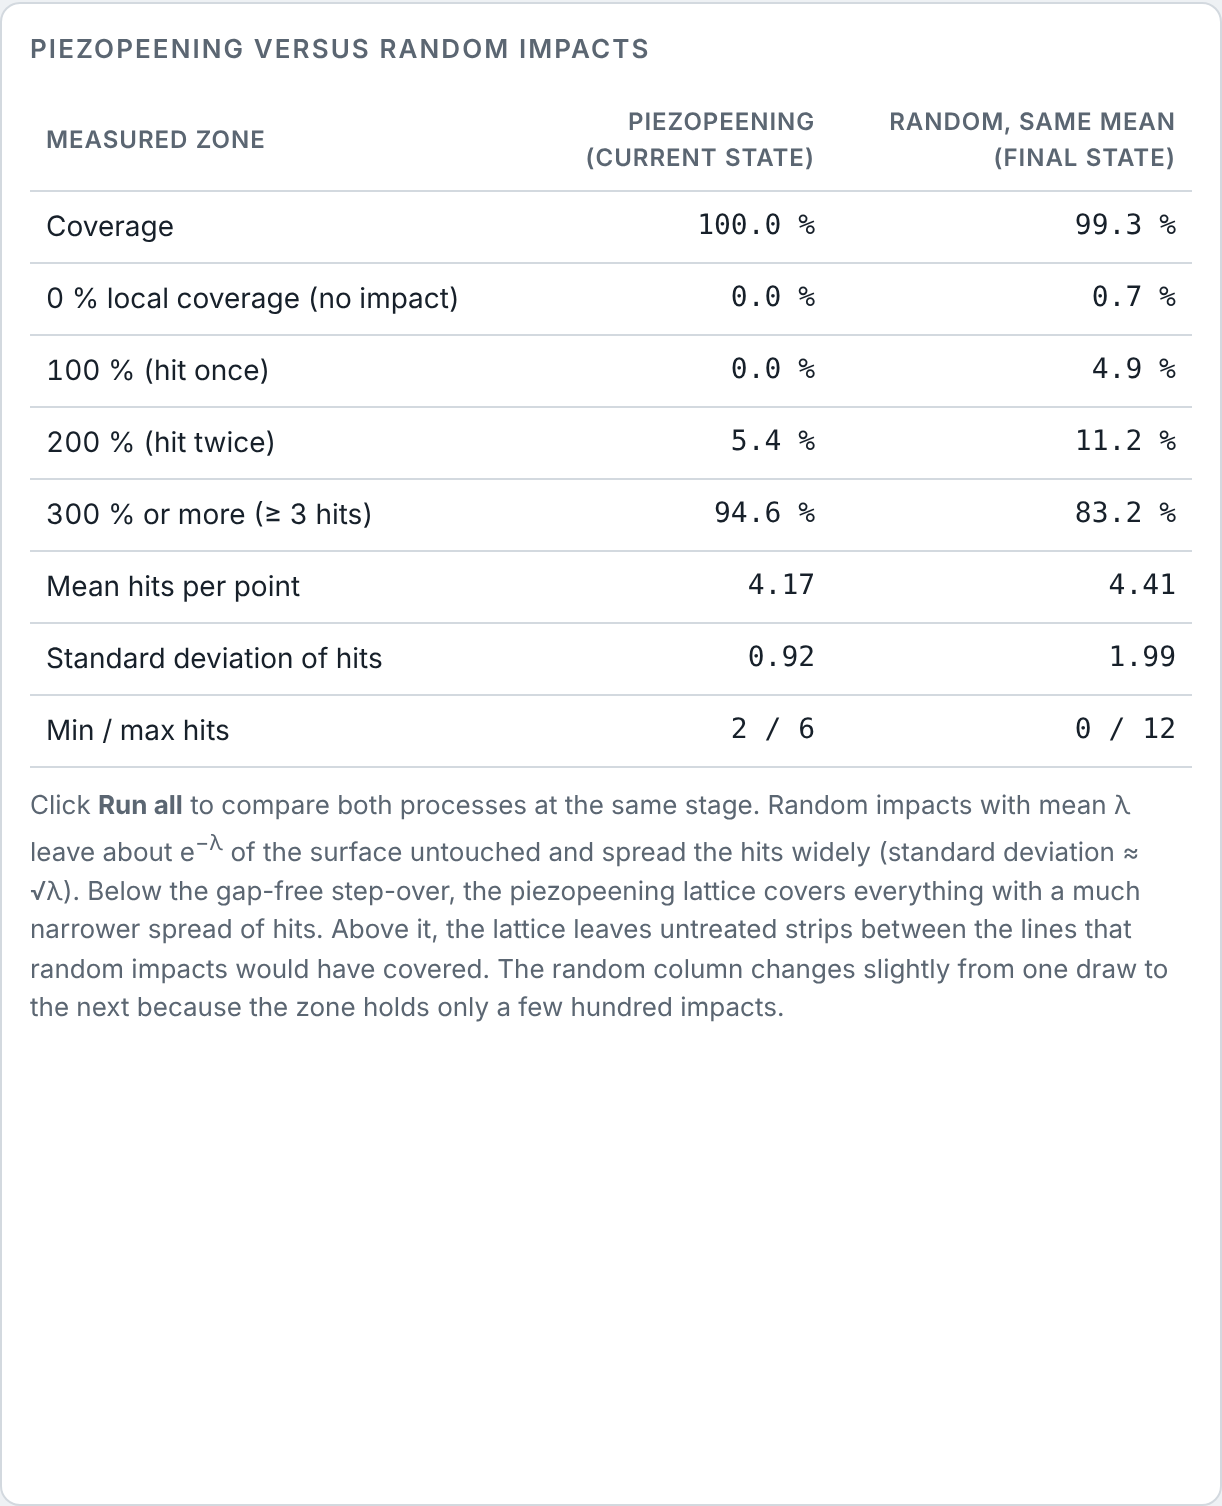
\includegraphics[width=\linewidth]{img/sec9.png}\caption{Comparison table.}\end{subfigure}
\caption{Same mean, very different spread.}
\end{figure}

\section{One-pass coverage versus step-over}

\begin{figure}[H]
\centering
\begin{subfigure}{0.48\linewidth}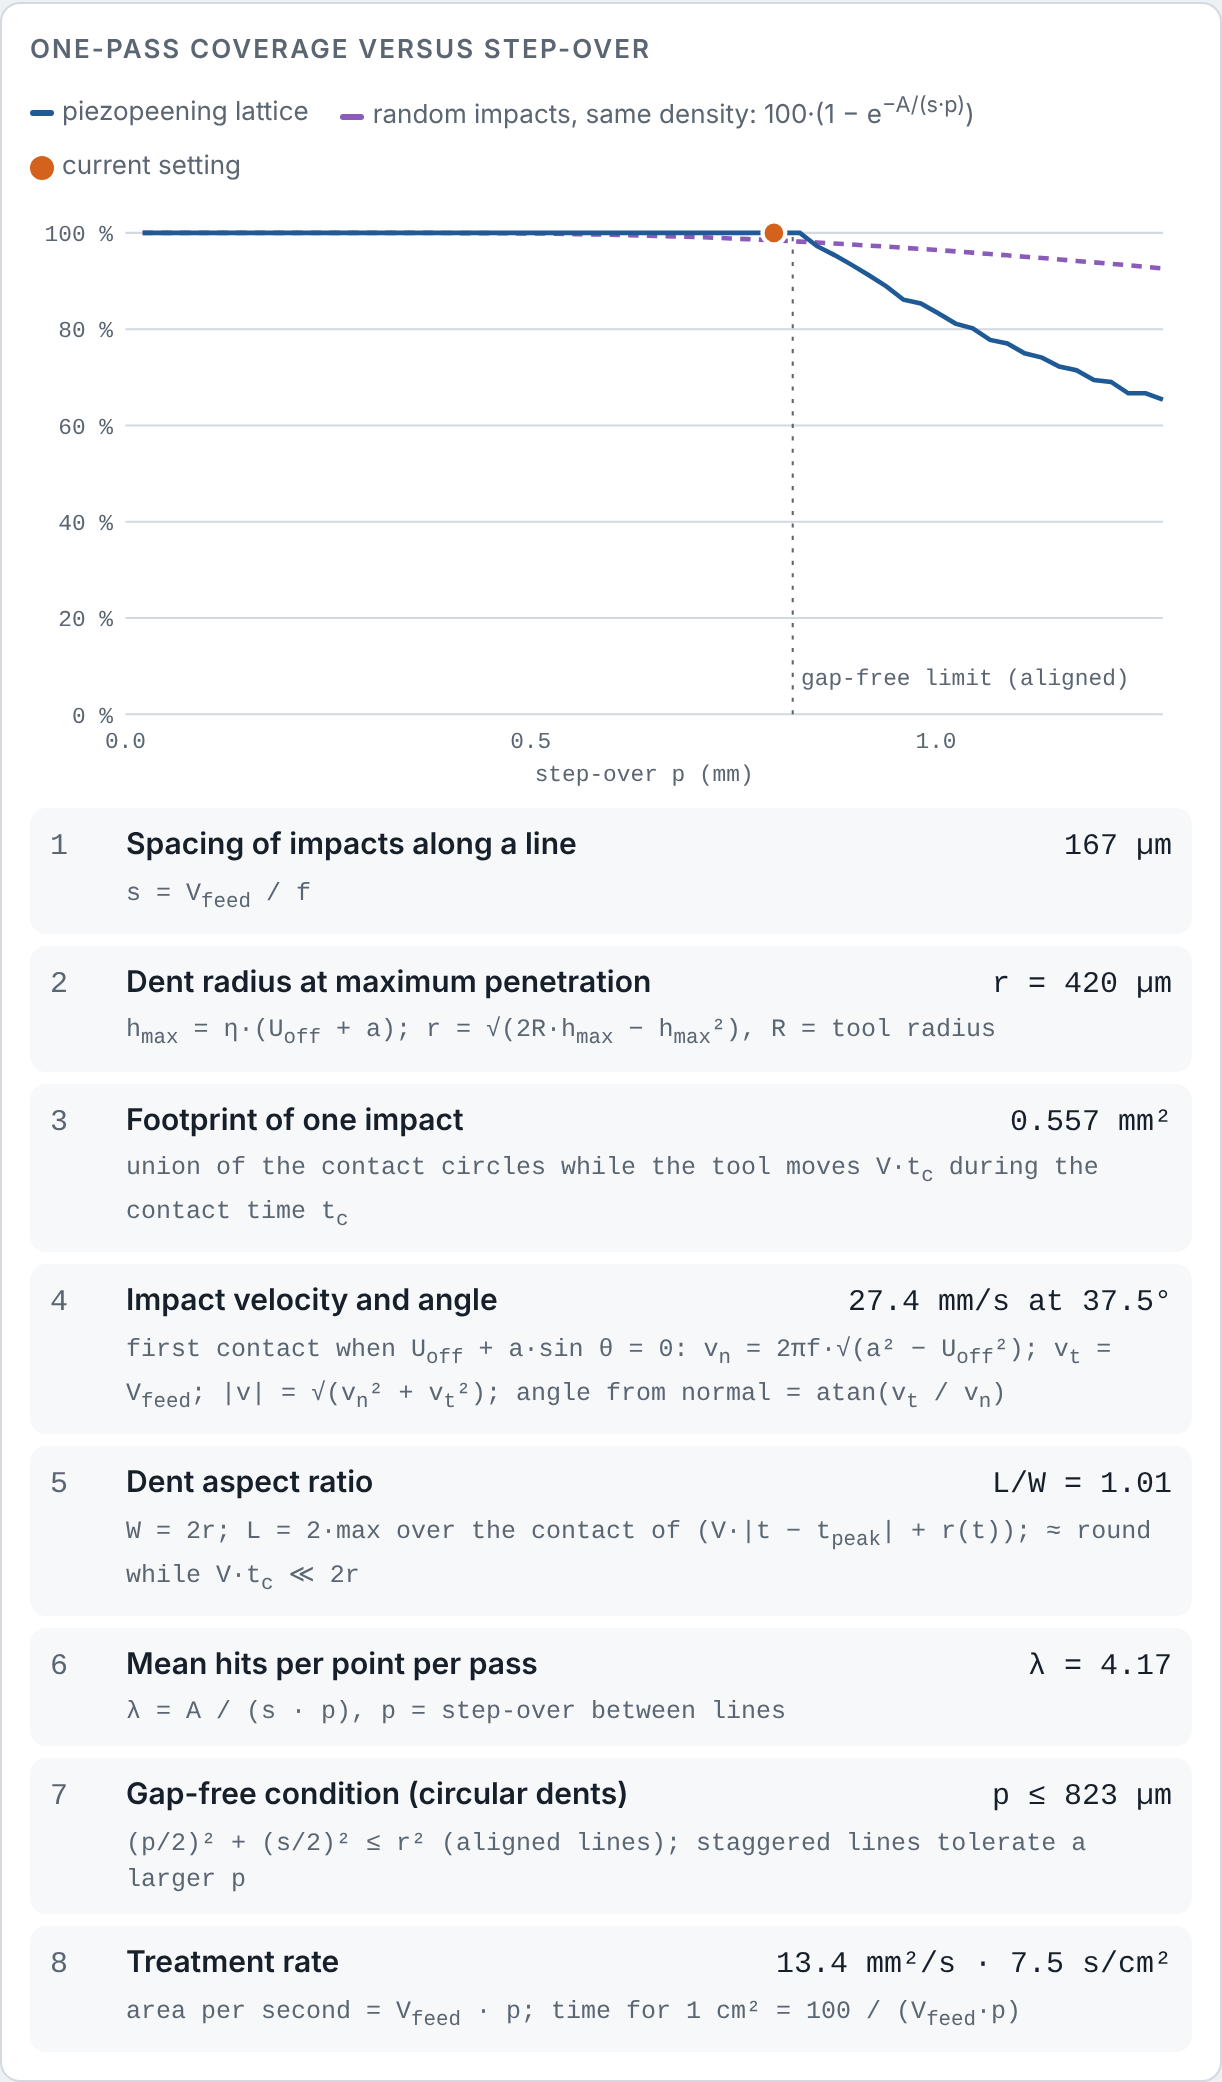
\includegraphics[width=\linewidth]{img/sec11.png}\caption{Chart and calculation chain.}\end{subfigure}\hfill
\begin{subfigure}{0.48\linewidth}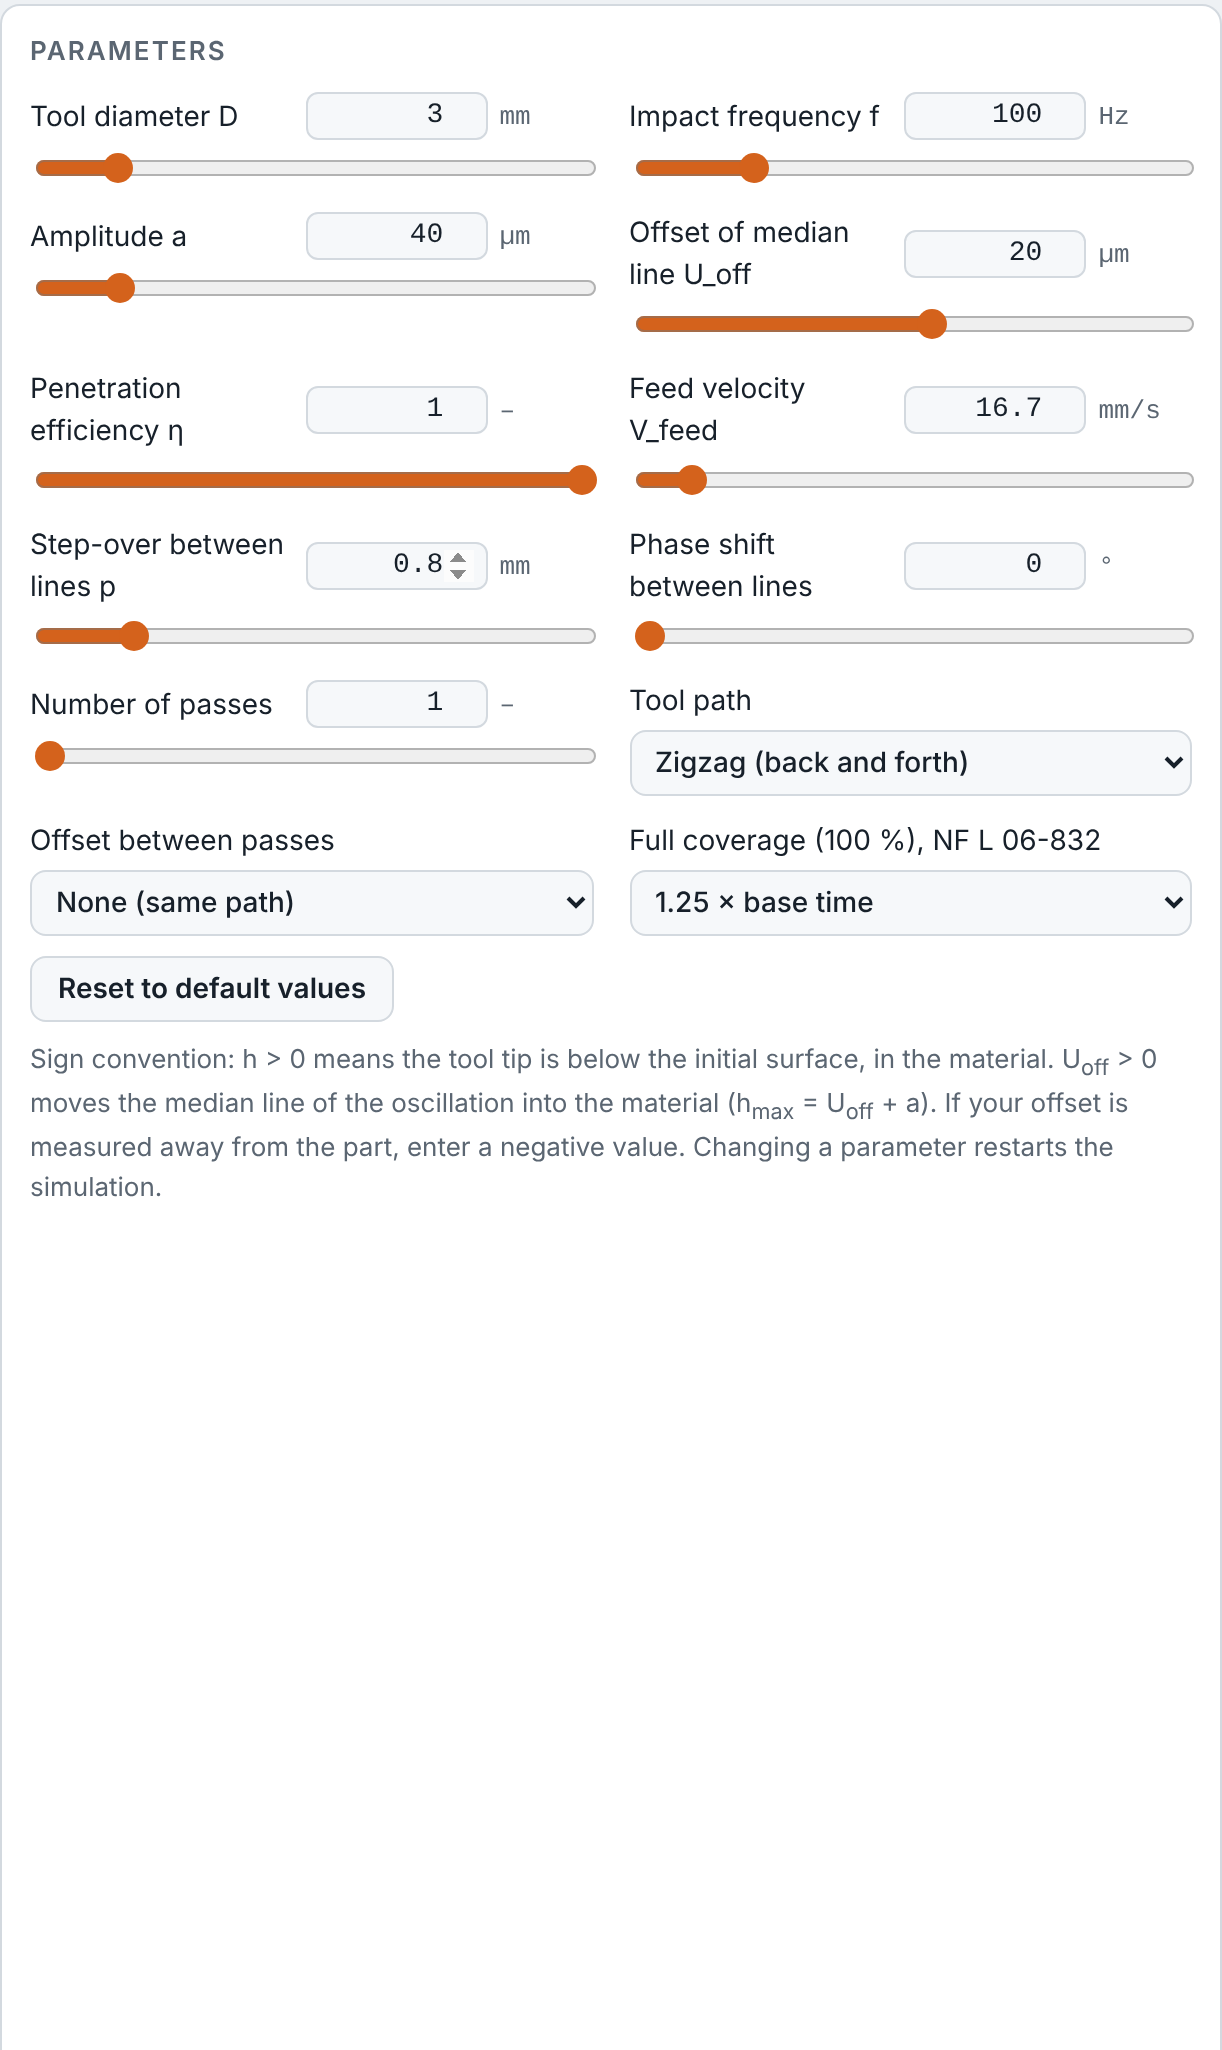
\includegraphics[width=\linewidth]{img/sec10.png}\caption{Parameters.}\end{subfigure}
\caption{The last two panels.}
\end{figure}

The chart plots, against $p$, the one-pass coverage of the lattice (solid line, computed on the periodic cell) and of random impacts with the same density, $100\bigl(1-e^{-A/(sp)}\bigr)$ (dashed). The lattice stays at 100\,\% up to the gap-free limit, then drops quickly; random impacts never reach 100\,\% but degrade slowly. The orange dot is the current setting.

\paragraph{Calculation chain.}
\begin{enumerate}[nosep,label=c\arabic*]
\item spacing of impacts along a line, $s=V/f$;
\item dent radius at maximum penetration, $r=\sqrt{2Rh_\mathrm{max}-h_\mathrm{max}^2}$;
\item footprint of one impact, $A$ (union of the contact circles while the tool moves $Vt_c$);
\item mean hits per point per pass, $\lambda=A/(sp)$;
\item gap-free condition, $p\le2\sqrt{r^2-(s/2)^2}$;
\item treatment rate, $Vp$, and time for \SI{1}{cm^2};
\item dent aspect ratio $L/W$;
\item impact velocity $|v|$ and its angle.
\end{enumerate}

\section{Every parameter}\label{sec:params}

\begin{longtable}{@{}p{3.9cm}p{1.1cm}p{2.0cm}p{1.9cm}p{5.2cm}@{}}
\toprule
\textbf{Parameter} & \textbf{Unit} & \textbf{Range} & \textbf{Default} & \textbf{Effect}\\ \midrule\endhead
Tool diameter $D$ & mm & 0.5 -- 20 & 3 & Larger tool, larger dents at the same depth.\\
Impact frequency $f$ & Hz & 1 -- 500 & 100 & $s=V/f$; more impacts per mm, rounder dents.\\
Amplitude $a$ & µm & 1 -- 300 & 40 & Stroke; sets $v_n$ and, with $U_\mathrm{off}$, the depth.\\
Offset of median line $U_\mathrm{off}$ & µm & $-300$ -- 300 & 20 & $>0$: median line inside the material. Sets the regime (none / impacts / continuous) and the contact time.\\
Penetration efficiency $\eta$ & -- & 0.05 -- 1 & 1 & Fraction of the motion that indents the surface.\\
Feed velocity $V$ & mm/s & 0.5 -- 200 & 16.7 & $s=V/f$; elongated dents at high $V$.\\
Step-over $p$ & mm & 0.02 -- 5 & 0.8 & Spacing of the lines; gaps above the gap-free limit.\\
Phase shift $\varphi$ & ° & 0 -- 360 & 0 & Shift of the impacts from one line to the next.\\
Number of passes $N$ & -- & 1 -- 10 & 1 & Repeats the treatment.\\
Tool path & -- & 2 choices & zigzag & Zigzag or one way.\\
Offset between passes & -- & 2 choices & none & None or half pitch ($p/2$, $s/2$).\\
Full coverage (100\,\%) & -- & 2 choices & 1.25 × base & NF~L~06-832 factor 1.25, or 100\,\% = base time.\\
\bottomrule
\end{longtable}
\noindent Changing a parameter restarts the simulation; \ui{Reset to default values} restores the defaults.

\section{Every result displayed}\label{sec:reads}

\begin{longtable}{@{}p{4.4cm}p{7.2cm}p{2.6cm}@{}}
\toprule
\textbf{Readout} & \textbf{Meaning and formula} & \textbf{Default}\\ \midrule\endhead
\multicolumn{3}{@{}l}{\emph{Top view}}\\
\ui{Lines done / total} & lines travelled / lines of all passes & 7 / 7\\
\ui{Impacts made} & number of dents & 238\\
\ui{Measured coverage} & share of the measured zone with $\ge1$ dent & 100.0\,\%\\
\ui{Predicted coverage (1 pass, lattice)} & coverage of the periodic cell & 100.0\,\%\\
\ui{Base time $t_b$ (98\,\% dented)} & first time 98\,\% of the zone is dented & 0.96 pass\\
\ui{Coverage (NF L 06-832)} & dented area up to $t_b$, then time-based & 98.3\,\%\\
\multicolumn{3}{@{}l}{\emph{Kinematics}}\\
\ui{Impact spacing s} & $V/f$ & 167\,µm\\
\ui{Max penetration} $h_\mathrm{max}$ & $\eta(U_\mathrm{off}+a)$ & 60.0\,µm\\
\ui{Dent radius r} & $\sqrt{2Rh_\mathrm{max}-h_\mathrm{max}^2}$ & 420\,µm\\
\ui{Contact time per cycle} & $t_c=(\theta_2-\theta_1)/(2\pi f)$ & 6.67 ms (67\,\%)\\
\ui{Normal impact velocity} $v_n$ & $2\pi f\sqrt{a^2-U_\mathrm{off}^2}$ & 21.8 mm/s\\
\ui{Tangential velocity} $v_t$ & $V$ & 16.7 mm/s\\
\ui{Resultant impact velocity} & $\sqrt{v_n^2+v_t^2}$ & 27.4 mm/s\\
\ui{Impact angle from the normal} & $\arctan(v_t/v_n)$ & 37.5°\\
\ui{Tool travel during contact} & $Vt_c$ & 111\,µm\\
\ui{Dent length L / width W} & along / across the feed & 845 / 840\,µm\\
\ui{Dent aspect ratio} & $L/W$ & 1.01 (round)\\
\ui{Footprint area A} & area of the union of contact circles & 0.557 mm²\\
\ui{Mean hits per point per pass} & $A/(sp)$ & 4.17\\
\multicolumn{3}{@{}l}{\emph{Hits}}\\
\ui{Mean hits per point} & mean count in the zone & 4.17\\
\ui{Min / max hits} & extreme counts & 2 / 6\\
\ui{Never-hit surface} & share with 0 hit & 0.0\,\%\\
\ui{Share 0 / 100 / 200 / $\ge$300\,\%} & share hit 0, 1, 2, $\ge3$ times & 0 / 0 / 5.4 / 94.6\\
\multicolumn{3}{@{}l}{\emph{Depth}}\\
\ui{Max / mean depth} & in the measured zone & 60.0 / 41.2\,µm\\
\ui{Shallowest point} & minimum depth & 4.8\,µm\\
\ui{Peak-to-valley} & max $-$ min depth & 55.1\,µm\\
\ui{Ridge between lines} & $H(p)$ & 54.3\,µm\\
\ui{Scallop between impacts} & $H(s)$ & 2.3\,µm\\
\multicolumn{3}{@{}l}{\emph{Roughness}}\\
\ui{Ra, Rq, Rp, Rv, Rt, Rz, Rsk, Rku, RSm} & 2D, four profiles (Section~\ref{sec:rough}) & 13.90\,µm\ldots\\
\ui{Sa, Sq, Ssk, Sku, Sp, Sv, Sz, Sdq, Sdr} & 3D, measured zone & 13.90\,µm\ldots\\
\multicolumn{3}{@{}l}{\emph{Comparison (random column)}}\\
\ui{Coverage}, \ui{0\,\% share} & random process, same density & 98.5, 1.5\,\%\\
\ui{Standard deviation of hits} & lattice / random ($\approx\sqrt\lambda$) & 0.92 / 2.00\\
\ui{Min / max hits} & random & 0 / 14\\
\bottomrule
\end{longtable}

\section{Things to try}

\begin{center}
\small
\begin{tabular}{@{}lccccl@{}}
\toprule
Change from the defaults & $r$ (µm) & $L/W$ & $\lambda$ & coverage & Comment\\ \midrule
none & 420 & 1.01 & 4.17 & 100 & random 98.5\,\%\\
$p=1.2$ mm & 420 & 1.01 & 2.78 & 71.1 & beyond gap-free limit; random 93.6\,\%\\
$V=100$ mm/s & 420 & 1.22 & -- & 82.5 & $s=1$ mm, elongated, 77.7° from normal\\
$V=200$ mm/s & 420 & 1.79 & -- & 59.7 & very elongated\\
$U_\mathrm{off}=-20$ µm & 244 & -- & -- & 57.2 & $h_\mathrm{max}=20$ µm, contact 33\,\%\\
$U_\mathrm{off}=-50$ µm & -- & -- & 0 & 0 & no contact\\
$U_\mathrm{off}=60$ µm & -- & groove & 6.85 & 100 & continuous contact, $W=1.08$ mm\\
$\eta=0.6$ & 327 & -- & -- & 80.4 & $h_\mathrm{max}=36$ µm\\
one way & 420 & 1.01 & 4.17 & 100 & same dents\\
$\varphi=180°$, $p=1.0$ mm & 420 & 1.01 & -- & 83.6 & staggered lines\\
$N=2$, half pitch, $p=1.2$ & 420 & 1.01 & -- & 100 & gaps filled; NF 99.2\,\%\\
$f=300$ Hz & 420 & -- & 12.44 & 100 & $s=56$ µm, 14.3° from normal\\ \bottomrule
\end{tabular}
\end{center}
\noindent(coverage = measured coverage in \%; ``--'' = not recorded here, read it on the page.)

\begin{trybox}
\begin{itemize}[nosep,leftmargin=*]
\item Increase $p$ slowly from 0.8 mm: watch the one-pass chart leave 100\,\% just above the gap-free limit (823\,µm), while the random curve hardly moves.
\item Set $p=\SI{1.2}{mm}$, then $N=2$ with \ui{Half pitch}: the second pass fills the gaps.
\item Set $N=3$: the dented area stays at 100\,\% while the coverage (NF~L~06-832) rises to 249\,\%.
\item Halve the step-over: $R_a$ across the feed falls from 13.9 to 3.4\,µm, while along the feed it does not change.
\item Raise $V$ to 100 mm/s: the dents become oval, the impact angle grows and the page warns about ploughing.
\item Move $U_\mathrm{off}$ from $-50$ to $+60$\,µm: no contact, short impacts, long impacts, continuous groove.
\item Compare the ridge heights across ($H(p)$) and along ($H(s)$) the feed: the waviness of the surface is set by the step-over.
\end{itemize}
\end{trybox}

\section{Assumptions and limits}

Rigid spherical tool and perfectly plastic indentation: the dent is the trace of the sphere, with no elastic recovery, no pile-up and no front lip; the contact radius follows the geometry $r=\sqrt{2Rh-h^2}$. The tool motion is a pure sine, unaffected by the contact force (the efficiency $\eta$ is a global correction). Flat part, constant feed and frequency, straight lines. The coverage and the number of hits describe the dented surface; they are not a measurement of the mechanical effect (residual stresses, hardening), which depends on the energy of each impact. The page is an educational tool; it does not replace process qualification.

\appendix
\section{Symbols}
\begin{tabular}{@{}ll@{\qquad}ll@{}}
$D,R$ & tool diameter, radius & $f$ & impact frequency\\
$a$ & amplitude & $U_\mathrm{off}$ & offset of the median line\\
$\eta$ & penetration efficiency & $h(t)$ & tool tip below the surface\\
$h_\mathrm{max}$ & maximum penetration & $t_c$ & contact time per cycle\\
$v_n,v_t$ & normal, tangential velocity & $V$ & feed velocity\\
$s$ & spacing of impacts, $V/f$ & $p$ & step-over\\
$\varphi$ & phase shift between lines & $N$ & number of passes\\
$r$ & dent radius & $L,W$ & dent length, width\\
$A$ & footprint area & $\lambda$ & mean hits per point\\
$H(e)$ & ridge height at spacing $e$ & & \\
\end{tabular}

\vfill
\noindent\small Code: MIT licence. Documentation: CC BY 4.0. Related tools: \url{https://rkubler.github.io/shotpeening/}.

\end{document}
